\documentclass[a4paper,12pt]{report}
\usepackage[left=2cm,right=2cm,top=2cm,bottom=3cm]{geometry}

%stuff I've added
\usepackage[utf8]{inputenc}
\usepackage{graphicx}% Include figure files
% \usepackage{dcolumn}% Align table columns on decimal point
% \usepackage{bm}% bold math
\usepackage{acronym}
\usepackage{physics}
% \usepackage{layouts}
\usepackage{acronym}
\usepackage{lipsum} 

\usepackage{amsmath}
\usepackage{amssymb}
\usepackage{svg}
\usepackage{comment}
\usepackage{placeins}
\usepackage{float}
\floatplacement{figure}{H} % the default figure placement specifier

\usepackage{hyperref}
\usepackage{cleveref}
\usepackage{bookmark}

\usepackage{pdfpages} % To be able to include pdfs in the appendix

\usepackage[version=4]{mhchem} % for chemical formulas

\usepackage[style=numeric, 
sorting=none,
hyperref=true]{biblatex}
\addbibresource{entire_zotero_library.bib}

\def\[#1\]{\begin{equation}#1\end{equation}}


% Exrta symbol commands
\newcommand{\tex}[1]{\expval{#1}} %Thermal expectation value
\newcommand{\qex}[1]{\expval{#1}} %Quantum expectation value
\newcommand{\Z}{\mathcal{Z}} %Partition function
\newcommand{\T}{\mathcal{T}} %MCMC Transition function
\newcommand{\A}{\mathcal{A}} %MCMC Acceptance function
\newcommand{\p}{\mathcal{P}} %MCMC Proposal distribution
\newcommand{\nfi}{n^f_i} %FK number operators of f electrons
\newcommand{\nfj}{n^f_j} %FK number operators of f electrons
\newcommand{\s}{\vec{s}} %used to refer to states of the spin system

\usepackage{orcidlink}

%for code blocks
\usepackage{listings}
\usepackage{xcolor}

\definecolor{codegreen}{rgb}{0,0.6,0}
\definecolor{codegray}{rgb}{0.5,0.5,0.5}
\definecolor{codepurple}{rgb}{0.58,0,0.82}
\definecolor{backcolour}{rgb}{0.95,0.95,0.92}
\definecolor{urlblue}{HTML}{007bff}

\lstdefinestyle{mystyle}{
    backgroundcolor=\color{backcolour},   
    commentstyle=\color{codegreen},
    keywordstyle=\color{magenta},
    numberstyle=\tiny\color{codegray},
    stringstyle=\color{codepurple},
    basicstyle=\ttfamily\footnotesize,
    breakatwhitespace=false,         
    breaklines=true,                 
    captionpos=b,                    
    keepspaces=true,                 
    numbers=left,                    
    numbersep=5pt,                  
    showspaces=false,                
    showstringspaces=false,
    showtabs=false,                  
    tabsize=2
}

\lstset{style=mystyle}
%endfor code blocks

% \begin{acronym}
    \newacro{FK}{Falikov-Kimball}
    \newacro{CDW}[CDW]{charge-density wave}
    \newacro{MCMC}{Markov chain Monte Carlo}
    \newacro{ED}{Exact Diagonalisation}
    \newacro{TMM}{Transfer Matrix Methods}
    \newacro{IPR}{Inverse Participation Ratio}
    \newacro{DOS}{density of states}
    \newacro{FTPT}{finite temperature phase transition}
    \newacro{LRI}{Long-Range Ising}
% \end{acronym}

\hypersetup{
    colorlinks = true,
    linkcolor  = black,
    citecolor  = black,
    urlcolor   = urlblue,
}

\urlstyle{same}

\usepackage{wrapfig}
\usepackage{floatflt}

%stuff that came in the template

\usepackage{graphicx}
\usepackage{verbatim}
\usepackage{latexsym}
\usepackage{mathchars}
\usepackage{setspace}

\input{blocked.sty}
\input{uhead.sty}
\input{boxit.sty}
\pagestyle{empty}

%

\makeatletter  %to avoid error messages generated by "\@". Makes Latex treat "@" like a letter

% \linespread{1.5} % enable to go back to 1.5 line spacing
\def\submitdate#1{\gdef\@submitdate{#1}}

\def\maketitle{
  \begin{titlepage}{
    %\linespread{1.5}
    \Large Imperial College of Science, Technology and Medicine \\
    %\linebreak
    Department of Physics
    \rm
    \vskip 3in
    \Large \bf \@title \par
  }
  \vskip 0.3in
  \par
  {\Large \@author}
  \vskip 4in
  \par
  Submitted in part fulfilment of the requirements for the degree of 
  \linebreak
  Doctor of Philosophy in Physics of Imperial College of Science, Technology and Medicine \@submitdate
  \vfil
  \end{titlepage}
}

\def\titlepage{
  \newpage
  \centering
  \linespread{1}
  \normalsize
  \vbox to \vsize\bgroup\vbox to 9in\bgroup
}
\def\endtitlepage{
  \par
  \kern 0pt
  \egroup
  \vss
  \egroup
  \cleardoublepage
}

\def\abstract{
  \pagenumbering{arabic}
  \begin{center}{
    \large\bf Abstract}
  \end{center}
  \small
  %\def\baselinestretch{1.5}
  % \linespread{1.5}
  \normalsize
}
\def\endabstract{
  \par
}

\newenvironment{acknowledgements}{
  \cleardoublepage
  \begin{center}{
    \large \bf Acknowledgements}
  \end{center}
  \small
  % \linespread{1.5}
  \normalsize
}{\cleardoublepage}
\def\endacknowledgements{
  \par
}

\newenvironment{dedication}{
  \cleardoublepage
  \begin{center}{
    \large \bf Dedication}
  \end{center}
  \small
  % \linespread{1.5}
  \normalsize
}{\cleardoublepage}
\def\enddedication{
  \par
}

\def\preface{
    % \pagenumbering{roman}
    \pagestyle{plain}
    % \doublespacing
}

\def\body{
    \pagestyle{plain}
    \cleardoublepage    
    \setlength{\parskip}{1.1ex}
    \tableofcontents
    % \cleardoublepage
    % \pagestyle{uheadings}
    % \listoftables
    % \pagestyle{plain}
    % \cleardoublepage

    \listoffigures
    \cleardoublepage

    \pagestyle{fancy}
    \setlength{\parskip}{2ex plus 0.5ex minus 0.2ex}
    \setlength{\parindent}{0pt}
}

\makeatother  %to avoid error messages generated by "\@". Makes Latex treat "@" like a letter

\newcommand{\ipc}{{\sf ipc}}

\newcommand{\Prob}{\bbbp}
\newcommand{\Real}{\bbbr}
% \newcommand{\real}{\Real}
\newcommand{\Int}{\bbbz}
\newcommand{\Nat}{\bbbn}

\newcommand{\NN}{{\sf I\kern-0.14emN}}   % Natural numbers
\newcommand{\ZZ}{{\sf Z\kern-0.45emZ}}   % Integers
\newcommand{\QQQ}{{\sf C\kern-0.48emQ}}   % Rational numbers
\newcommand{\RR}{{\sf I\kern-0.14emR}}   % Real numbers
\newcommand{\KK}{{\cal K}}
\newcommand{\OO}{{\cal O}}
\newcommand{\AAA}{{\bf A}}
\newcommand{\HH}{{\bf H}}
\newcommand{\II}{{\bf I}}
\newcommand{\LL}{{\bf L}}
\newcommand{\PP}{{\bf P}}
\newcommand{\PPprime}{{\bf P'}}
\newcommand{\QQ}{{\bf Q}}
\newcommand{\UU}{{\bf U}}
\newcommand{\UUprime}{{\bf U'}}
\newcommand{\zzero}{{\bf 0}}
\newcommand{\ppi}{\mbox{\boldmath $\pi$}}
\newcommand{\aalph}{\mbox{\boldmath $\alpha$}}
\newcommand{\bb}{{\bf b}}
\newcommand{\ee}{{\bf e}}
\newcommand{\mmu}{\mbox{\boldmath $\mu$}}
\newcommand{\vv}{{\bf v}}
\newcommand{\xx}{{\bf x}}
\newcommand{\yy}{{\bf y}}
\newcommand{\zz}{{\bf z}}
\newcommand{\oomeg}{\mbox{\boldmath $\omega$}}
\newcommand{\res}{{\bf res}}
\newcommand{\cchi}{{\mbox{\raisebox{.4ex}{$\chi$}}}}
%\newcommand{\cchi}{{\cal X}}
%\newcommand{\cchi}{\mbox{\Large $\chi$}}

% Logical operators and symbols
\newcommand{\imply}{\Rightarrow}
\newcommand{\bimply}{\Leftrightarrow}
\newcommand{\union}{\cup}
\newcommand{\intersect}{\cap}
\newcommand{\boolor}{\vee}
\newcommand{\booland}{\wedge}
\newcommand{\boolimply}{\imply}
\newcommand{\boolbimply}{\bimply}
\newcommand{\boolnot}{\neg}
\newcommand{\boolsat}{\!\models}
\newcommand{\boolnsat}{\!\not\models}


% \newcommand{\op}[1]{\mathrm{#1}}
% \newcommand{\s}[1]{\ensuremath{\mathcal #1}}

% Properly styled differentiation and integration operators
\newcommand{\diff}[1]{\mathrm{\frac{d}{d\mathit{#1}}}}
\newcommand{\diffII}[1]{\mathrm{\frac{d^2}{d\mathit{#1}^2}}}
\newcommand{\intg}[4]{\int_{#3}^{#4} #1 \, \mathrm{d}#2}
\newcommand{\intgd}[4]{\int\!\!\!\!\int_{#4} #1 \, \mathrm{d}#2 \, \mathrm{d}#3}

% Large () brackets on different lines of an eqnarray environment
\newcommand{\Leftbrace}[1]{\left(\raisebox{0mm}[#1][#1]{}\right.}
\newcommand{\Rightbrace}[1]{\left.\raisebox{0mm}[#1][#1]{}\right)}

% Funky symobols for footnotes
\newcommand{\symbolfootnote}{\renewcommand{\thefootnote}{\fnsymbol{footnote}}}
% now add \symbolfootnote to the beginning of the document...

\newcommand{\normallinespacing}{\renewcommand{\baselinestretch}{1.5} \normalsize}
\newcommand{\mediumlinespacing}{\renewcommand{\baselinestretch}{1.2} \normalsize}
\newcommand{\narrowlinespacing}{\renewcommand{\baselinestretch}{1.0} \normalsize}
\newcommand{\bump}{\noalign{\vspace*{\doublerulesep}}}
\newcommand{\cell}{\multicolumn{1}{}{}}
\newcommand{\spann}{\mbox{span}}
\newcommand{\diagg}{\mbox{diag}}
\newcommand{\modd}{\mbox{mod}}
\newcommand{\minn}{\mbox{min}}
\newcommand{\andd}{\mbox{and}}
\newcommand{\forr}{\mbox{for}}
\newcommand{\EE}{\mbox{E}}

\newcommand{\deff}{\stackrel{\mathrm{def}}{=}}
\newcommand{\syncc}{~\stackrel{\textstyle \rhd\kern-0.57em\lhd}{\scriptstyle L}~}

\def\coop{\mbox{\large $\rhd\!\!\!\lhd$}}
\newcommand{\sync}[1]{\raisebox{-1.0ex}{$\;\stackrel{\coop}{\scriptscriptstyle
#1}\,$}}

\newtheorem{definition}{Definition}[chapter]
\newtheorem{theorem}{Theorem}[chapter]

%%% For things that pandoc uses
\newenvironment{Shaded}{}{}
\newenvironment{Highlighting}{}{}
\newcommand{\AlertTok}[1]{\textcolor[rgb]{1.00,0.00,0.00}{\textbf{#1}}}
\newcommand{\AnnotationTok}[1]{\textcolor[rgb]{0.38,0.63,0.69}{\textbf{\textit{#1}}}}
\newcommand{\AttributeTok}[1]{\textcolor[rgb]{0.49,0.56,0.16}{#1}}
\newcommand{\BaseNTok}[1]{\textcolor[rgb]{0.25,0.63,0.44}{#1}}
\newcommand{\BuiltInTok}[1]{#1}
\newcommand{\CharTok}[1]{\textcolor[rgb]{0.25,0.44,0.63}{#1}}
\newcommand{\CommentTok}[1]{\textcolor[rgb]{0.38,0.63,0.69}{\textit{#1}}}
\newcommand{\CommentVarTok}[1]{\textcolor[rgb]{0.38,0.63,0.69}{\textbf{\textit{#1}}}}
\newcommand{\ConstantTok}[1]{\textcolor[rgb]{0.53,0.00,0.00}{#1}}
\newcommand{\ControlFlowTok}[1]{\textcolor[rgb]{0.00,0.44,0.13}{\textbf{#1}}}
\newcommand{\DataTypeTok}[1]{\textcolor[rgb]{0.56,0.13,0.00}{#1}}
\newcommand{\DecValTok}[1]{\textcolor[rgb]{0.25,0.63,0.44}{#1}}
\newcommand{\DocumentationTok}[1]{\textcolor[rgb]{0.73,0.13,0.13}{\textit{#1}}}
\newcommand{\ErrorTok}[1]{\textcolor[rgb]{1.00,0.00,0.00}{\textbf{#1}}}
\newcommand{\ExtensionTok}[1]{#1}
\newcommand{\FloatTok}[1]{\textcolor[rgb]{0.25,0.63,0.44}{#1}}
\newcommand{\FunctionTok}[1]{\textcolor[rgb]{0.02,0.16,0.49}{#1}}
\newcommand{\ImportTok}[1]{#1}
\newcommand{\InformationTok}[1]{\textcolor[rgb]{0.38,0.63,0.69}{\textbf{\textit{#1}}}}
\newcommand{\KeywordTok}[1]{\textcolor[rgb]{0.00,0.44,0.13}{\textbf{#1}}}
\newcommand{\NormalTok}[1]{#1}
\newcommand{\OperatorTok}[1]{\textcolor[rgb]{0.40,0.40,0.40}{#1}}
\newcommand{\OtherTok}[1]{\textcolor[rgb]{0.00,0.44,0.13}{#1}}
\newcommand{\PreprocessorTok}[1]{\textcolor[rgb]{0.74,0.48,0.00}{#1}}
\newcommand{\RegionMarkerTok}[1]{#1}
\newcommand{\SpecialCharTok}[1]{\textcolor[rgb]{0.25,0.44,0.63}{#1}}
\newcommand{\SpecialStringTok}[1]{\textcolor[rgb]{0.73,0.40,0.53}{#1}}
\newcommand{\StringTok}[1]{\textcolor[rgb]{0.25,0.44,0.63}{#1}}
\newcommand{\VariableTok}[1]{\textcolor[rgb]{0.10,0.09,0.49}{#1}}
\newcommand{\VerbatimStringTok}[1]{\textcolor[rgb]{0.25,0.44,0.63}{#1}}
\newcommand{\WarningTok}[1]{\textcolor[rgb]{0.38,0.63,0.69}{\textbf{\textit{#1}}}}
\frenchspacing

\ifdefined\linespacing
  \renewcommand{\baselinestretch}{\linespacing} 
\fi

\input{latexdiff_preamble}

\begin{document}

\title{\LARGE {\bf The Long-Range Falicov-Kimball
Model and the Amorphous Kitaev Model \\
[0.2em]\smaller{}Quantum Many-Body Systems I have known and loved}\\
 \vspace*{6mm}
}

\author{Thomas Hodson\\\vspace{10mm}
\includegraphics[width=.4\textwidth,height=.4\textheight]{figure_code/logo/logo}
\vspace{-0.4\textheight}
\vspace{10mm}
}
\submitdate{October 2022}

% \normallinespacing

\maketitle

\preface

%The abstract page
\addcontentsline{toc}{chapter}{Abstract}
\begin{abstract}
\input{build/latex/0_Preface/0.1_Abstract}
\end{abstract}

% the page with versions, declaration of originality and copyright
\include{build/latex/0_Preface/0.2_Declarations}

% the Acknodledgemnet page
\cleardoublepage
\addcontentsline{toc}{chapter}{Acknowledgements}
\begin{acknowledgements}
\input{build/latex/0_Preface/0.3_Aknowledgements}
\end{acknowledgements}

% the dedication page
\cleardoublepage
% \begin{dedication}
\vspace*{100mm} % about one third of the vertical of an A4 page
\begin{center}To Kathrin.\end{center}
% \end{dedication}

\body

\hypersetup{
  linkcolor  = urlblue,
  citecolor  = black,
  urlcolor   = urlblue,
  }

\hypertarget{chap:1-introduction}{\chapter{Introduction}}
\begin{refsection}
\begin{Shaded}
\begin{Highlighting}[]
\OperatorTok{\%\%}\NormalTok{html}
\end{Highlighting}
\end{Shaded}

\hypertarget{outline}{%
\section{Outline}\label{outline}}

This thesis is composed of two main studies of separate but related physical models, The Falikov-Kimball Model and the Kitaev-Honeycomb Model. In this chapter I will discuss the overarching motivations for looking at these two physical models. I will then review the literature and methods that are common to both models.

In Chapter 2 I will look at the Falikov-Kimball model. I will review what it is and why we would want to study it. I'll survey what is already known about it and identify the gap in the research that we aim to fill, namely the model's behaviour in one dimension. I'll then introduce the modified model that we came up with to close this gap. I will present our results on the thermodynamic phase diagram and localisation properties of the model

In Chapter 3 I'll study the Kitaev Honeycomb Model, following the same structure as Chapter 2 I will motivate the study, survey the literature and identify a gap. I'll introduce our Amorphous Kitaev Model designed to fill this gap and present the results.

Finally in chapter 4 I will summarise the results and discuss what implications they have for our understanding interacting many-body quantum systems.

One of the most interesting and perhaps surprising features of many body physics is the existence of distinct phases of matter.

Why does liquid turn to ice? Well there are two key ingredients. First we need a system composed of a large number of objects and second we need those objects to interact with eachother.

It turns out that the more objects there are, the greater the effect that their interactions has on the whole. A hundred \(H_2O\) molecules can't actually form the nice regular structure that characterises ice, instead you'd get more of a blob. However, any human scale amount of water contains an unimaginable huge number of molecules.

Phases come about when the interactions between individuals components serve the reinforce

When a many body, interacting system can display radically different properties depending on the system parameters

\textbf{Themes} - many body - interactions - quantum - topology - disorder

\begin{itemize}
\item
  quasiparticles
\item
  topological order
\item
  protected edge states
\item
  Abelian and non-Abelian anyons
\item
  localisation
\item
  length scales
\end{itemize}

\hypertarget{interacting-quantum-many-body-systems}{%
\section{Interacting Quantum Many Body Systems}\label{interacting-quantum-many-body-systems}}

\textbf{Interacting Many-Body Quantum Systems}

\emph{Figure showing energy scales of interest on a log plot}

Condensed matter is called condensed because in the scheme of things it is the physics of objects that are quite cold. Working at high energies allows one to probe deeper and deeper into the substructure of things, from atoms to nuclei to nucleons to quarks to gluons. At one stage the behaviour may be well described by talking of protons and neutrons binding together, while at the next it is necessary to bring gluons and quarks into the picture.

It is perhaps not surprising then, that going to lower energies produces the reverse effect. If we start with a gas of atoms and cool it, we will get a solid. In that solid, we find that the relevant objects are not even particles in the sense that one might imagine, they are instead collective motions (or excitations) of the constituent particles which we call quasiparticles.

Sometimes it is said that quasiparticles are a bit like waves on the ocean. And in a sense they are, however because they live in the quantum realm they are far weirder and more diverse than ocean waves. Their quantumness gives them a distinct identity and indivisibility that waves do not have. They can interact both directly and, more strangely, simply by moving around one another.

I will be looking at the behaviour of electrons in crystalline and amorphous materials. The ingredients that I will consider are:

\begin{itemize}
\tightlist
\item
  Interactions between particles
\item
  Disorder or randomness in the system
\item
  Symmetries of the system
\item
  The dimensionality of the system
\item
  Temperature
\item
  While perhaps obvious, the fact of there being many bodies is itself a key ingredient.
\end{itemize}

In keeping with the theme of trying to keep things simple, I will use the tight binding approximation of electrons moving against a fixed atomic background potential. I will discuss the advantages and disadvantages of this approximation in the next chapter but for now let's say that it captures enough of the essence of reality to explain many physical phenomena.

\href{venndiagram}{Modelling reality requires three basic ingredients: we need quantum objects, we need a lot of them and we need them to interact. However these three properties taken together make for an almost completely intractable problem. Many approaches to modelling reality in condensed matter can be thought of as tackling this problem by going after one of these ingredients. Diagrammatic methods set interactions to zero and add them back in perturbatively. Mean field methods get rid of the many bodies. Condensed matter theorists are excited about ADS/CFT correspondences because the can map interacting quantum problems onto classical ones. The models I study in this thesis could be classified into this scheme as follows. The FK model model contains many interacting bodies but what makes it tractable is that we have classical species interacting with quantum ones, because the quantum particles never interact among one another we can still make progress with simulations. The Kitaev Honeycomb Model and our generalisations of it essentially rely on a similar trick, though in this case the classical degrees of freedom are emergent they still serve to decouple the quantum degrees of freedom from interacting with one another.}

\textbf{Spin-Orbit Coupling}

Electronic wavefunctions can be understood as quantum extensions of

This can be loosely understood as a consequence of that fact that electrons are `orbiting' their host nucleus and in doing so they are moving with respect to an electric field generated by the positive charge of the nucleus. The electric field looks like a magnetic field in the rest frame of the electron and this magnetic field couples to the magnetic spin moment of the electron.

This analogy is wrong on many levels but it suffices to understand that there should be such an effect.

Going one level deeper we can estimate the scale of the effect by combining the non-relativistic quantum theory of a spin in a magnetic field with the classical relativistic electromagnetism prediction for how the electric field turns into a magnetic field in the rest frame of the electron. This gets us within a factor to two of the correct answer but it fails to account for an extra relativistic effect called Thomas Precession \textbf{cite}.

The next level would be to compute this effect within relativistic QM using the Dirac equation. And finally, we could do the full calculation within Quantum Electrodynamics where we would find tiny corrections that come about from virtual processes involving particle-antiparticle pairs that spring form from the vacuum.

\hypertarget{mott-insulators-and-the-hubbard-model}{%
\section{Mott Insulators and The Hubbard Model}\label{mott-insulators-and-the-hubbard-model}}

\begin{fignos:no-prefix-figure-caption}

\begin{figure}
\centering
\includegraphics{5d575ef5-9414-4f30-a2cc-9a2b8cd44cc0.png}
\caption{image.png}
\end{figure}

\end{fignos:no-prefix-figure-caption}

These are easiest to understand within the context of the Hubbard model, if we take spin \(1/2\) fermions hopping on the lattice with hopping parameter \(t\) and interaction strength \(U\) \[ H = -t \sum_{\langle i,j \rangle \alpha} c^\dagger_{i\alpha} c_{j\alpha} + \sum_i c^\dagger_{i\uparrow} c_{i\downarrow}\]

where \(c^\dagger_{i\alpha}\) creates a spin \(\alpha\) electron at site \(i\). Pauli exclusion prevents two electrons with the same spin being at the same site so which is why the interaction term only couples opposite spin electrons. The only physically relevant parameter here is \(U/t\) which compared the interaction strength \(U\) to the importance of kinetic energy \(t\).

In the free fermion limit \(U/t = 0\), we can just find the single particle eigenstates and fill them up to the fermi level. The many body ground state has no particular electron-electron correlations.

In the interacting limit, \(t/U = 0\), there's no hopping so electrons just site wherever we put them. We can fill the system up until there is one electron per site without any energy penalty at all. The maximum we can fill the system up to

\begin{fignos:no-prefix-figure-caption}

\begin{figure}
\centering
\includegraphics{f25fb28d-4239-4184-9a9e-b6704189019d.png}
\caption{Stolen from https://arxiv.org/pdf/1701.07056.pdf}
\end{figure}

\end{fignos:no-prefix-figure-caption}

\textbf{Condensed Matter Theory}

\href{energy_scales}{A collection of important energy scales plotted on a logarithmic scale. We can take room temperature somewhere in the middle of the plot as a reference point. Moving towards higher energies we'll gradually probe deeper into the smaller and smaller structures of the universe, atoms, protons, quarks etc. While going to lower energies we move to larger and larger scales and objects made up of progressively more and more components.}

There's a common joke among condensed matter physicists that the field is the study of dirt. I quite like this definition because within the average handful of dirt you're not unlikely to find crystals, metals, glasses and all manner of other things that condensed matter physicists like to study.

The second reason I like this definition is that dirt is complex. It has structure at many scales. It is heterogeneous and contaminated with traces of all manner of things. It's dirty. When I talk about real physical things like this, I will use the word systems.

On the other hand, we have mathematical tools at our disposal to describe and understand the world around us. I'll use the word model whenever I am talking about these mathematical constructions that describe the real word.

This leads one of the central tensions of condensed matter theory: our models are ill-equipped to deal with the complexity inherent in the real world. We may be able to write down a mathematical description of a handful of dirt, but we wouldn't be able to solve it. And a model we cannot solve will not further our understanding.

So what do we do? Well, we simplify. We try to ask ``What are the essential ingredients required to model this particular phenomenon?''

Answering this question lets us write down simpler models that we have a better chance of being able to solve. And by paring the description down to the bare minimum, it also gives us a better chance of being able to understand why these systems behave the way they do.

I will therefore be focusing on highly simplified models of reality, each containing only a few ingredients. I will then investigate what phenomena can be observed in these models and try to relate the findings to more messy reality.

\hypertarget{spin-liquids}{%
\section{Spin Liquids}\label{spin-liquids}}

\hypertarget{exactly-solvable-models}{%
\section{Exactly Solvable Models}\label{exactly-solvable-models}}

\begin{Shaded}
\begin{Highlighting}[]

\end{Highlighting}
\end{Shaded}

\printbibliography[heading=subbibintoc]
\end{refsection}

\hypertarget{chap:2-background}{\chapter{Background}}
\backgroundsetup{scale = 1, angle = 0, opacity = 1,
  contents = {\includegraphics[width=297mm, height=297mm]{figure_code/chapter_2_background_pdfa}}}
\BgThispage
\begin{refsection}
\hypertarget{the-falikov-kimball-model}{%
\section{The Falikov Kimball Model}\label{the-falikov-kimball-model}}

\hypertarget{the-model}{%
\subsection{The Model}\label{the-model}}

discuss CDW phase of 2d model as motivation for studying 1d phase with long range forces

\hypertarget{particle-hole-symmetry}{%
\subsubsection{Particle Hole Symmetry}\label{particle-hole-symmetry}}

\hypertarget{phase-diagram}{%
\subsection{Phase Diagram}\label{phase-diagram}}

\hypertarget{long-range-ising-models}{%
\subsection{Long Range Ising Models}\label{long-range-ising-models}}

\begin{Shaded}
\begin{Highlighting}[]

\end{Highlighting}
\end{Shaded}

\hypertarget{bg-hkm-model}{%
\section{The Kitaev Honeycomb Model}\label{bg-hkm-model}}

\hypertarget{fig:intro_figure_by_hand}{%
\begin{figure}
\centering
\includegraphics[width=1\textwidth,height=\textheight]{figure_code/amk_chapter/intro/honeycomb_zoom/intro_figure_by_hand}
\caption[{The Kitaev Honeycomb Model}]{\textbf{(a)} The Kitaev honeycomb model is defined on a honeycomb lattice. The special feature of the honeycomb lattice that makes the model solvable is that each vertex is joined by exactly three bonds, i.e.~the lattice is trivalent. One of three labels is assigned to each bond (x,y,z) here represented by colour. \textbf{(b)}. After transforming to the Majorana representation we get an emergent gauge degree of freedom \(u_{jk} = \pm 1\) that lives on each bond, the bond variables. These are antisymmetric, \(u_{jk} = -u_{kj}\), so we represent them graphically with arrows on each bond that point in the direction that \(u_{jk} = +1\) \textbf{(c)}. The Majorana transformation can be visualised as breaking each spin into four Majoranas \(b_i^x,\;b_i^y,\;b_i^z,\;c_i\). The x, y and z Majoranas then pair along the bonds forming conserved \(\mathbb{Z}_2\) bond operators \(u_{jk} = \langle i b_i^\alpha b_j^\alpha \rangle\). The remaining \(c_i\) operators form an effective quadratic Hamiltonian \(H = \frac{i}{4} \sum_{\langle i,j\rangle_\alpha} 2J^{\alpha} u_{ij} \hat{c}_i \hat{c}_j\).}
\label{fig:intro_figure_by_hand}
\end{figure}
}

\hypertarget{the-spin-hamiltonian}{%
\subsection{The Spin Hamiltonian}\label{the-spin-hamiltonian}}

This section introduces the Kitaev honeycomb (KH) model. The KH model is an exactly solvable model of interacting spin\(-1/2\) spins on the vertices of a honeycomb lattice. Each bond in the lattice is assigned a label \(\alpha \in \{ x, y, z\}\) and that bond couple two spins along the \(\alpha\) axis. See \cref{fig:intro_figure_by_hand} for a diagram of the setup.

This gives us the Hamiltonian \begin{equation}\protect\hypertarget{eq:bg-kh-model}{}{ H =  - \sum_{\langle j,k\rangle_\alpha} J^{\alpha}\sigma_j^{\alpha}\sigma_k^{\alpha}, }\label{eq:bg-kh-model}\end{equation} where \(\sigma^\alpha_j\) is the \(\alpha\) component of a Pauli matrix acting on site \(j\) and \(\langle j,k\rangle_\alpha\) is a pair of nearest-neighbour indices connected by an \(\alpha\)-bond with exchange coupling \(J^\alpha\). Kitaev introduced this model in his seminal 2006 paper~\autocite{kitaevAnyonsExactlySolved2006}.

The KH can arise as the result of strong spin-orbit couplings in, for example, the transition metal based compounds~\autocite{Jackeli2009,HerrmannsAnRev2018,Winter2017,TrebstPhysRep2022,Takagi2019}. The model is highly frustrated: each spin would like to align along a different direction with each of its three neighbours but this cannot be achieved even classically~\autocite{chandraClassicalHeisenbergSpins2010,selaOrderbydisorderSpinorbitalLiquids2014}. This frustration leads the model to have a quantum spin liquid (QSL) ground state, a complex many body state with a high degree of entanglement but no long range magnetic order even at zero temperature. While the possibility of a QSL ground state was suggested much earlier~\autocite{andersonResonatingValenceBonds1973}, the KH model was the first exactly solvable models of the QSL state. The KH model has a rich ground state phase diagram with gapless and gapped phases, the latter supporting fractionalised quasiparticles with both Abelian and non-Abelian quasiparticle excitations. Anyons have been the subject of much attention because, among other reasons, they can be braided through spacetime to achieve noise tolerant quantum computations~\autocite{freedmanTopologicalQuantumComputation2003}. At finite temperature the KH model undergoes a phase transition to a thermal metal state~\autocite{selfThermallyInducedMetallic2019}. The KH model can be solved exactly via a mapping to Majorana fermions. This mapping yields an extensive number of static \(\mathbb Z_2\) fluxes tied to an emergent gauge field with the remaining fermions are governed by a free fermion hamiltonian.

This section will go over the standard model in detail, first discussing \protect\hyperlink{the-spin-model}{the spin model}, then detailing the transformation to a \protect\hyperlink{the-majorana-model}{Majorana hamiltonian} that allows a full solution while enlarging the Hamiltonian. We will discuss the properties of the \protect\hyperlink{an-emergent-gauge-field}{emergent gauge fields} and the projector. The \protect\hyperlink{sec:anyons}{next section} will discuss anyons, topology and the Chern number, using the Kitaev model as an explicit example of these topics. Finally will then discuss the ground state found via Lieb's theorem as well as work on generalisations of the ground state to other lattices. Finally we will look at the \protect\hyperlink{ground-state-phases}{phase diagram}.

\hypertarget{the-spin-model}{%
\subsection{The Spin Model}\label{the-spin-model}}

\hypertarget{fig:visual_kitaev_1}{%
\begin{figure}
\centering
\includegraphics[width=1\textwidth,height=\textheight]{figure_code/amk_chapter/visual_kitaev_1}
\caption[{A Visual Intro to the Kitaev Model}]{A visual introduction to the Kitaev Model.}
\label{fig:visual_kitaev_1}
\end{figure}
}

As discussed in the introduction, spin hamiltonians like that of the Kitaev model arise in electronic systems as the result the balance of multiple effects~\autocite{TrebstPhysRep2022}. For instance, in certain transition metal systems with \(d^5\) valence electrons, crystal field and spin-orbit couplings conspire to shift and split the \(d\) orbitals into moments with spin \(j = 1/2\) and \(j = 3/2\). Of these, the bandwidth \(t\) of the \(j= 1/2\) band is small, meaning that even relatively meagre electron correlations (such those induced by the \(U\) term in the Hubbard model) can lead to the opening of a Mott gap. From there we have a \(j = 1/2\) Mott insulator whose effective spin-spin interactions are again shaped by the lattice geometry and spin-orbit coupling leading some materials to have strong bond-directional Ising-type interactions~\autocite{jackeliMottInsulatorsStrong2009,khaliullinOrbitalOrderFluctuations2005}. In the Kitaev Model the bond directionality refers to the fact that the coupling axis \(\alpha\) in terms like \(\sigma_j^{\alpha}\sigma_k^{\alpha}\) is strongly bond dependent.

In the spin hamiltonian \cref{eq:bg-kh-model} we can already tease out a set of conserved fluxes that will be key to the model's solution. These fluxes are the expectations of Wilson loop operators

\[\hat{W}_p = \prod_{\langle i,j\rangle_\alpha\; \in\; p} \sigma_i^{\alpha}\sigma_j^{\alpha},\]

the products of bonds winding around a closed path \(p\) on the lattice. These operators commute with the Hamiltonian and so have no time dynamics. The winding direction does not matter so long as it is fixed. By convention we will always use clockwise. Each closed path on the lattice is associated with a flux. The number of conserved quantities grows linearly with system size and is thus extensive, this is a common property for exactly solvable systems and can be compared to the heavy electrons present in the Falikov-Kimball model. The square of two loop operators is one so any contractible loop can be expressed as a product of loops around plaquettes of the lattice, as in \cref{fig:stokes_theorem}. For the honeycomb lattice the plaquettes are the hexagons. The expectations of \(\hat{W}_p\) through each plaquette, the fluxes, are therefore enough to describe the whole flux sector. We will focus on these fluxes, denoting them by \(\phi_i\). Once we have made the mapping to the Majorana Hamiltonian I will explain how these fluxes can be connected to an emergent \(B\) field which makes their interpretation as fluxes clear.

\hypertarget{fig:stokes_theorem}{%
\begin{figure}
\centering
\includegraphics[width=0.71\textwidth,height=\textheight]{figure_code/amk_chapter/stokes_theorem/stokes_theorem}
\caption[{We can construct arbitrary loops from plaquette fluxes.}]{In the Kitaev Honeycomb model, Wilson loop operators \(\hat{W}_p = \prod_{\langle i,j\rangle_\alpha\; \in\; p} \sigma_i^{\alpha}\sigma_j^{\alpha}\) can be composed via multiplication to produce arbitrary contractible loops. As a consequence we need only to keep track of the value of the flux through each plaquette \(\phi_i\). This relationship between the \(u_{ij}\) around a region and fluxes with one is evocative of Stokes' theorem for classical electromagnetism. In fact it turns out to be the exponential of it as we shall make explicit later.}
\label{fig:stokes_theorem}
\end{figure}
}

It is worth noting in passing that the effective Hamiltonian for many Kitaev materials incorporates a contribution from an isotropic Heisenberg term \(\sum_{i,j} \vec{\sigma}_i\cdot\vec{\sigma}_j\), this is referred to as the Heisenberg-Kitaev Model~\autocite{Chaloupka2010}. Materials for which the Kitaev term dominates are generally known as Kitaev Materials. See~\autocite{TrebstPhysRep2022} for a full discussion of Kitaev Materials.

As with the Falikov-Kimball model, the KH model has a extensive number of conserved quantities, the fluxes. As with the FK model it will make sense to work in the simultaneous eigenbasis of the fluxes and the Hamiltonian so that we can treat the fluxes like a classical degree of freedom. This is part of what makes the model tractable. We will find that the ground state of the model corresponds to some particular choice of fluxes. We will refer to local excitations away from the flux ground state as \emph{vortices}. In order to fully solve the model however, we must first move to a Majorana picture.

\hypertarget{the-majorana-model}{%
\subsection{The Majorana Model}\label{the-majorana-model}}

Majorana fermions are something like `half of a complex fermion' and are their own antiparticle. From a set of \(N\) fermionic creation \(f_i^\dagger\) and anhilation \(f_i\) operators we can construct \(2N\) Majorana operators \(c_m\). We can do this construction in multiple ways subject to only mild constraints required to keep the overall commutations relations correct~\autocite{kitaevAnyonsExactlySolved2006}. Majorana operators square to one but otherwise have standard fermionic commutation relations.

\(N\) spins can be mapped to \(N\) fermions with the well known Jordan-Wigner transformation and indeed this approach can be used to solve the Kitaev model~\autocite{chenExactResultsKitaev2008}. Here I will introduce the method Kitaev used in the original paper as this forms the basis for the results that will be presented in this thesis. Rather than mapping to \(N\) fermions, Kitaev maps to \(4N\) Majoranas, effectively \(2N\) fermions. In contrast to the Jordan-Wigner approach which makes fermions out of strings of spin operators in order to correctly produce fermionic commutation relations, the Kitaev transformation maps each spin locally to four Majoranas. The downside is that this enlarges the Hilbert space from \(2^N\) to \(4^N\). We will have to employ a projector \(\hat{P}\) to come back down to the physical Hilbert space later. As everything is local, I will drop the site indices \(ijk\) in expressions that refer to only a single site.

The mapping is defined in terms of four Majoranas per site \(b_i^x,\;b_i^y,\;b_i^z,\;c_i\) such that

\begin{equation}\protect\hypertarget{eq:bg-kh-mapping}{}{\tilde{\sigma}^x = i b^x c,\; \tilde{\sigma}^y = i b^y c,\; \tilde{\sigma}^z = i b^z c}\label{eq:bg-kh-mapping}\end{equation}

The tildes on the spin operators \(\tilde{\sigma_i^\alpha}\) emphasis that they live in this new extended Hilbert space and are only equivalent to the original spin operators after applying a projector \(\hat{P}\). The form of the projection operator can be understood in a few ways. From a group-theoretic perspective, before projection, the operators \(\{\tilde{\sigma}^x, \tilde{\sigma}^y, \tilde{\sigma}^z\}\) form a representation of the gamma group \(G_{3,0}\). The gamma groups \(G_{p,q}\) have \(p\) generators that square to the identity and \(q\) that square (roughly) to \(-1\). The generators otherwise obey standard anticommutation relations. The well known gamma matrices \(\{\gamma^0, \gamma^1, \gamma^2, \gamma^3\}\) represent \(G_{1,3}\) the quaternions \(G_{0,3}\) and the Pauli matrices \(G_{3,0}\).

The Pauli matrices, however, have the additional property that the \emph{chiral element} \(\sigma^x \sigma^y \sigma^z = \pmi\) is not fully determined by the group properties of \(G_{3,0}\) but it is equal to \(i\) in the Pauli matrices. Therefore to fully reproduce the algebra of the Pauli matrices we must project into the subspace where \(\tilde{\sigma}^x \tilde{\sigma}^y \tilde{\sigma}^z = +i\). The chiral element of the gamma matrices for instance \(\gamma_5 = i\gamma^0 \gamma^1 \gamma^2 \gamma^3\) is of central importance in quantum field theory. See~\autocite{petitjeanChiralityDiracSpinors2020} for more discussion of this group theoretic view.

So the projector must project onto the subspace where \(\tilde \sigma^x \tilde \sigma^y \tilde \sigma^z = i\). If we work this through we find that in general \(\tilde \sigma^x \tilde \sigma^y \tilde\sigma^z = iD\) where \(D = b^x b^y b^z c\) must be the identity for every site. In other words, we can only work with \emph{physical states} \(|\phi\rangle\) that satisfy \(D_i|\phi\rangle = |\phi\rangle\) for all sites \(i\). From this we construct an on-site projector \(P_i = \frac{1 + D_i}{2}\) and the overall projector is simply \(P = \prod_i P_i\).

Another way to see what this is doing physically is to explicitly construct the two intermediate fermionic operators \(f\) and \(g\) that give rise to these four Majoranas. Denoting a fermion state by \(|n_f, n_g\rangle\) the Hilbert space is the set \(\{|00\rangle,|01\rangle,|10\rangle,|11\rangle\}\). We can map these to Majoranas with, for example, this definition

\[\begin{aligned}
b^x = (f + f^\dagger),\;\;& b^y = -i(f - f^\dagger),\\
b^z = (g + g^\dagger),\;\;& c = -i(g - g^\dagger),
\end{aligned}\]

Working through the algebra we see that the operator \(D = b^x b^y b^z c\) is equal to the fermion parity \(D = -(2n_f - 1)(2n_g - 1) = \pm1\) where \(n_f,\; n_g\) are the number operators. So setting \(D = 1\) everywhere is equivalent to restricting to the \(\{|01\rangle,|10\rangle\}\) though we could equally well have used the other one.

Expanding the product \(\prod_i P_i\) out, we find that the projector corresponds to a symmetrisation over \(\{u_{ij}\}\) states within a flux sector and and overall fermion parity \(\prod_i D_i\). The significance of this is that an arbitrary many body state can be made to have non-zero overlap with the physical subspace via the addition or removal of just a single fermion. This implies that in the thermodynamic limit the projection step is not generally necessary to extract physical results, see~\autocite{pedrocchiPhysicalSolutionsKitaev2011} or \protect\hyperlink{app-the-projector}{appendix A.5} for more details.

We can now rewrite the spin hamiltonian in Majorana form with the caveat that they are only strictly equivalent after projection. The Ising interactions \(\sigma_j^{\alpha}\sigma_k^{\alpha}\) decouple into the form \(-i (i b^\alpha_i b^\alpha_j) c_i c_j\). We factor out the \emph{bond operators} \(\hat{u}_{ij} = i b^\alpha_i b^\alpha_j\) which are Hermitian and, remarkably, commute with the Hamiltonian and each other.

\[\begin{aligned}
\tilde{H} &=  - \sum_{\langle i,j\rangle_\alpha} J^{\alpha}\tilde{\sigma}_i^{\alpha}\tilde{\sigma}_j^{\alpha}\\
          &=  i \sum_{\langle i,j\rangle_\alpha} J^{\alpha} \hat{u}_{ij} \hat{c}_i \hat{c}_j
\end{aligned}\]

The bond operators \(\hat{u}_{ij}\) square to one so have eigenvalues \(\pm1\). As they're conserved we will work in their eigenbasis and take off the hats in the Hamiltonian.

\begin{equation}\protect\hypertarget{eq:bg-kh-maj-model}{}{\begin{aligned}
H &=  i \sum_{\langle i,j\rangle_\alpha} J^{\alpha} u_{ij} \hat{c}_i \hat{c}_j
\end{aligned}}\label{eq:bg-kh-maj-model}\end{equation}

\hypertarget{the-fermion-problem}{%
\subsection{The Fermion Problem}\label{the-fermion-problem}}

We now have a quadratic Hamiltonian, \cref{eq:bg-kh-maj-model}, coupled to a classical field \(u_{ij}\). What follows is relatively standard theory for quadratic Hamiltonians~\autocite{BlaizotRipka1986}.

Because of the antisymmetry \(J^{\alpha} u_{ij}\), the eigenvalues of \cref{eq:bg-kh-maj-model} come in pairs \(\pm \epsilon_m\). We organise the eigenmodes of \(H\) into pairs, such that \(b_m\) and \(b_m'\) have energies \(\epsilon_m\) and \(-\epsilon_m\). The transformation \(Q\) \[(c_1, c_2... c_{2N}) Q = (b_1, b_1', b_2, b_2' ... b_{N}, b_{N}')\] puts the Hamiltonian into normal mode form \[\tilde{H}_u = \frac{i}{2} \sum_m \epsilon_m b_m b_m'.\]

The determinant of \(Q\) appears when evaluating the projector explicitly, otherwise, the \(b_m\) are merely an intermediate step. From them, we form fermionic operators \[ f_i = \tfrac{1}{2} (b_m + ib_m')\] with their associated number operators \(n_i = f^\dagger_i f_i\). These let us write the Hamiltonian neatly as

\[ \tilde{H}_u = \sum_m \epsilon_m (n_m - \tfrac{1}{2}).\]

The energy of the ground state \(|n_m = 0\rangle\) of the many body system at fixed \(\{u_{ij}\}\) is

\[E_{u,0} = -\frac{1}{2}\sum_m \epsilon_m \]

and we can construct any state from a particular choice of \(n_m = 0,1\).

\hypertarget{an-emergent-gauge-field}{%
\subsection{An Emergent Gauge Field}\label{an-emergent-gauge-field}}

We have transformed the spin Hamiltonian into a Majorana hamiltonian \(H = i \sum_{\langle i,j\rangle_\alpha} J^{\alpha} u_{ij} \hat{c}_i \hat{c}_j\) describing the dynamics of a classical field \(u_{ij}\) and Majoranas \(c_i\). It is natural to ask how the classical field \(u_{ij}\) relates to the fluxes of the original spin model. We can evaluate the fluxes \(\phi_i\) in terms of the bond operators

\begin{equation}\protect\hypertarget{eq:flux-majorana}{}{\phi_i = \prod_{\langle j,k\rangle \in \mathcal{P}_i} i u_{jk}.}\label{eq:flux-majorana}\end{equation}

\hypertarget{fig:gauge_symmetries}{%
\begin{figure}
\centering
\includegraphics[width=1\textwidth,height=\textheight]{figure_code/amk_chapter/intro/gauge_symmetries/gauge_symmetries}
\caption[{Gauge Symmetries}]{A honeycomb lattice with edges in light grey, along with its dual, the triangle lattice in light blue. The vertices of the dual lattice are the faces of the original lattice and, hence, are the locations of the vortices. (Left) The action of the gauge operator \(D_j\) at a vertex is to flip the value of the three \(u_{jk}\) variables (black lines) surrounding site \(j\). The corresponding edges of the dual lattice (red lines) form a closed triangle. (Middle) Composing multiple adjacent \(D_j\) operators produces a large closed dual loop or multiple disconnected dual loops. Dual loops are not directed like Wilson loops. (Right) A non-contractable loop which cannot be produced by composing \(D_j\) operators. All three operators can be thought of as the action of a vortex-vortex pair that is created, one of them is transported around the loop, and then the two annihilate again. Note that every plaquette has an even number of \(u_{ij}\)s flipped on its edge. Therefore, all retain the same flux \(\phi_i\).}
\label{fig:gauge_symmetries}
\end{figure}
}

In addition, the bond operators form a highly degenerate description of the system. The operators \(D_i = b^x_i b^y_i b^z_i c_i\) commute with \(H\) forming a set of local symmetries. The action of \(D_i\) on a state is to flip the values of the three \(u_{ij}\) bonds that connect to site \(i\). This changes the bond configuration \(\{u_{ij}\}\) but leaves the flux configuration \(\{\phi_i\}\) unchanged. Physically, we interpret \(u_{ij}\) as a gauge field with a high degree of degeneracy and \(\{D_i\}\) as the set of gauge symmetries. The Majorana bond operators \(u_{ij}\) are an emergent, classical, \(\mathbb{Z}_2\) gauge field! The flux configuration \(\{\phi_i\}\) is what encodes physical information about the system without all the gauge degeneracy.

The ground state of the Kitaev Honeycomb model is the all one flux configuration \(\{\phi_i = +1\; \forall \; i\}\). This can be proven via Lieb's theorem~\autocite{lieb_flux_1994} which gives the lowest energy magnetic flux configuration for a system of electrons hopping in a magnetic field. Kitaev remarks in his original paper that he was not initially aware of the relevance of Lieb's 1994 result. This is not surprising because at first glance the two models seem quite different but the connection is quite instructive for understanding the Kitaev Model and its generalisations.

Lieb discusses a model of mobile electrons

\[H = \sum_{ij} t_{ij} c^\dagger_i c_j\]

where the hopping terms \(t_{ij} = |t_{ij}|\exp(i\theta_{ij})\) incorporate Aharanhov-Bohm (AB) phases~\autocite{aharonovSignificanceElectromagneticPotentials1959} \(\theta_{ij}\). The AB phases model the effect of a slowly varying magnetic field on the electrons through the integral of the magnetic vector potential \(\theta_{ij} = \int_i^j \vec{A} \cdot d\vec{l}\), a Peierls substitution~\autocite{peierlsZurTheorieDiamagnetismus1933}. If we map the Majorana form of the Kitaev model to Lieb's model we see that our \(t_{ij} = i J^\alpha u_{ij}\). The \(i u_{ij} = \pm i\) correspond to AB phases \(\theta_{ij} = \pi/2\) or \(3\pi/2\) along each bond.

\hypertarget{fig:regular_plaquettes}{%
\begin{figure}
\centering
\includegraphics[width=0.86\textwidth,height=\textheight]{figure_code/amk_chapter/intro/regular_plaquettes/regular_plaquettes}
\caption[{Plaquettes in the Kitaev Model}]{Lieb's theorem gives the ground state flux configuration for even sided plaquettes in systems with at least one translationally invariant direction~\autocite{lieb_flux_1994}. These labels correspond to the Kitaev fluxes \(\phi_i\) rather than the magnetic fluxes \(Q_i\) of Lieb's original paper (\(\phi_i = \exp{iQ_i}\)). Other work has extended Lieb's theorem numerically to arbitrary plaquettes,~\autocite{eschmannThermodynamicClassificationThreedimensional2020,Yao2009,eschmann2019thermodynamics,Peri2020}. The additional twofold degeneracy of the \(\pm i, \mp i\) terms is a consequence of the odd sided plaquettes breaking chiral symmetry. Chiral symmetry is spontaneously broken in the ground state~\autocite{Yao2009}.}
\label{fig:regular_plaquettes}
\end{figure}
}

Stokes' theorem tells us that the magnetic flux \(Q_m\) through a surface \(S\) is related to the line integral of \(\vec{A}\) along the boundary of the surface \(\partial S\) which in the discrete case reduces to the sum of the AB phases along the path. We can thus rewrite \cref{eq:flux-majorana} as

\begin{equation}\protect\hypertarget{eq:flux-magnetic}{}{\begin{aligned}
\phi_i &= \prod_{\mathcal{P}_i} i u_{jk}\\
       &= \prod_{\mathcal{P}_i} \exp{(i\theta_{jk}})\\
       &= \exp \left( i \sum_{\mathcal{P}_i} \theta_{jk} \right)\\
       &= \exp \left( i \oint_{\mathcal{P}_i} \vec{A} \cdot d\vec{l} \right)\\
       &= \exp \left( i Q_i \right)
\end{aligned}}\label{eq:flux-magnetic}\end{equation}

Thus we can interpret the fluxes \(\phi_i\) as the exponential of magnetic fluxes \(Q_m\) of some fictitious gauge field \(\vec{A}\) and the bond operators as \(i u_{ij} = \exp i \int_i^j \vec{A} \cdot d\vec{l}\). In this analogy to classical electromagnetism, the sets \(\{u_{ij}\}\) that correspond to the same \(\{\phi_i\}\) are all gauge equivalent as we have already seen via other means. The fact that fluxes can be written as products of bond operators and composed is a consequence of \cref{eq:flux-magnetic}. If the lattice contains odd plaquettes, as in the Yao-Kivelson model~\autocite{yaoExactChiralSpin2007}, the complex fluxes that appear are a sign that chiral symmetry has been broken.

In full, Lieb's theorem states that the ground state has magnetic flux \(Q_i = \sum_{\mathcal{P}_i}\theta_{ij} = \pi \; (\mathrm{mod} \;2\pi)\) for plaquettes with \(0 \; (\mathrm{mod}\;4)\) sides and \(0 \; (\mathrm{mod}\;2\pi)\) for plaquettes with \(2 \; (\mathrm{mod}\;4)\) sides. In terms of our fluxes, this means \(\phi = -1\) for squares, \(\phi = 1\) for hexagons and so on.

While Lieb's theorem is restricted to bipartite lattices with translational symmetry, other works has shown numerically that it tends to hold for more general lattices too~\autocite{eschmannThermodynamicClassificationThreedimensional2020,Yao2009,eschmann2019thermodynamics,Peri2020}. From this we find that the generalisation to odd sided plaquettes is similar but with an additional chiral symmetry, so \(\phi = \pm i\) for plaquettes with \(1 \; (\mathrm{mod}\;4)\) sides and \(\mp i\) for those with \(3 \; (\mathrm{mod}\;4)\) sides. Overall we can write \(\phi = -(\pm i)^{n_{\mathrm{sides}}}\). Later I will present numerical evidence that this rule continues to hold for general amorphous lattices.

Understanding \(u_{ij}\) as a gauge field provides another way to understand the action of the projector. The local projector \(P_i = \frac{1 + D_i}{2}\) applied to a state constructs a superposition of the original state and the gauge equivalent state linked to it by flipping the three \(u_{ij}\) around site \(i\). The overall projector \(P = \prod_i P_i\) can thus be understood as a symmetrisation over all gauge equivalent states, removing the gauge degeneracy introduced by the mapping from spins to Majoranas.

\hypertarget{fig:topological_fluxes}{%
\begin{figure}
\centering
\includegraphics[width=0.57\textwidth,height=\textheight]{figure_code/amk_chapter/topological_fluxes.png}
\caption[{Topological Fluxes}]{Wilson loops that wind the major or minor diameters of the torus measure flux winding through the hole of the doughnut/torus (red) or through the filling (green). If they made doughnuts which had both had a jam filling and a hole, this analogy would be a lot easier to make~\autocite{parkerWhyDoesThis}.}
\label{fig:topological_fluxes}
\end{figure}
}

A final but important point to mention is that the local fluxes \(\phi_i\) are not quite all there is. We've seen that products of \(\phi_i\) can be used to construct the flux associated with arbitrary contractible loops. On the plane contractible loops are all there is. However, on the torus we can construct two global fluxes \(\Phi_x\) and \(\Phi_y\) which correspond to paths tracing the major and minor axes. The four sectors spanned by the \(\pm1\) values of these fluxes are gapped away from one another but only by virtual tunnelling processes so the gap decays exponentially with system size~\autocite{kitaevAnyonsExactlySolved2006}. Physically \(\Phi_x\) and \(\Phi_y\) could be thought of as measuring the flux that threads through the hole of the doughnut. In general, surfaces with genus \(g\) have \(g\) `handles' and \(2g\) of these global fluxes. At first glance it may seem this would not have much relevance to physical realisations of the Kitaev model that will likely have a planar geometry with open boundary conditions. However these fluxes are closely linked to topology and the existence of anyonic quasiparticle excitations in the model, which we will discuss next.

\hypertarget{sec:anyons}{%
\subsection{Anyons, Topology and the Chern number}\label{sec:anyons}}

\hypertarget{fig:braiding}{%
\begin{figure}
\centering
\includegraphics[width=0.71\textwidth,height=\textheight]{figure_code/amk_chapter/braiding.png}
\caption[{Braiding in Two Dimensions}]{Worldlines of particles in two dimensions can become tangled or \emph{braided} with one another.}
\label{fig:braiding}
\end{figure}
}

To discuss different ground state phases of the KH model we must first review the topic of anyons and topology. The standard argument for the existence of Fermions and Bosons goes like this: the quantum state of a system must pick up a factor of \(\pm1\) if two identical particles are swapped. Only \(\pm1\) are allowed since swapping twice must correspond to the identity. This argument works in three dimensions for states without topological degeneracy, which seems to be true of the real world, but condensed matter systems are subject to no such constraints.

In gapped condensed matter systems, all equal time correlators decay exponentially with distance~\autocite{hastingsLiebSchultzMattisHigherDimensions2004}. Put another way, gapped systems support quasiparticles with a definite location in space and finite extent. As such it is meaningful to consider what would happen to the overall quantum state if we were to adiabatically carry out a series of swaps as described above. This is known as braiding. Recently, braiding in topological systems has attracted interest because of proposals to use ground state degeneracy to implement both passively fault tolerant and actively stabilised quantum computations~\autocite{kitaev_fault-tolerant_2003,poulinStabilizerFormalismOperator2005,hastingsDynamicallyGeneratedLogical2021}.

First we realise that in two dimensions, swapping identical particles twice is not topologically equivalent to the identity, see \cref{fig:braiding}. Instead it corresponds to encircling one particle around the other. This means we can in general pick up any complex phase \(e^{i\theta}\), hence the name \textbf{any}-ons upon exchange. These are known as Abelian anyons because complex multiplication commutes and hence the group of braiding operations forms an Abelian group.

The KH model has a topologically degenerate ground state with sectors labelled by the values of the topological fluxes \((\Phi_x\), \(\Phi_y)\). Consider the operation in which a quasiparticle pair is created from the ground state, transported around one of the non-contractible loops and then annihilated together, call them \(\mathcal{T}_{x}\) and \(\mathcal{T}_{y}\). These operations move the system around within the ground state manifold and they need not commute. This leads to non-Abelian anyons. As Kitaev points out, these operations are not specific to the torus: the operation \(\mathcal{T}_{x}\mathcal{T}_{y}\mathcal{T}_{x}^{-1}\mathcal{T}_{y}^{-1}\) corresponds to an operation in which none of the particles crosses the torus, rather one simply winds around the other, hence these effects are relevant even for the planar case.

In condensed matter systems, the existence of anyonic excitations automatically implies the system has topological ground state degeneracy on the torus~\autocite{einarssonFractionalStatisticsTorus1990} and indeed anyons and topology are intimately linked~\autocite{oshikawaTopologicalDegeneracyNonAbelian2007,Chung_Topological_quantum2010,yaoAlgebraicSpinLiquid2009}. The Chern number \(\nu\), a concept originally used to describe complex vector bundles in algebraic topology~\autocite{chernCharacteristicClassesHermitian1946}, has found use in physics as a powerful diagnostic tool for topological systems. Kitaev showed that there is a full classification of anyonic statistics in terms of \(\nu\;(\mathrm{mod}\;16)\) but relevant to us is that vortices in the KH model are Abelian when the Chern number is even and non-Abelian when the Chern number is odd. Non-Abelian statistics of the vortices in the KH model arise due to unpaired Majorana modes that are bound to them.

\hypertarget{ground-state-phases}{%
\subsection{Ground State Phases}\label{ground-state-phases}}

\hypertarget{fig:KH_phase_diagram}{%
\begin{figure}
\centering
\includegraphics[width=1\textwidth,height=\textheight]{figure_code/background_chapter/KH_phase_diagram}
\caption[{Kitaev Honeycomb Model Phase Diagram}]{Setting the energy scale of the Kitaev Model with the constraint that \(J_x + J_y + J_z = 1\) yields a triangular phase diagram where each of the corners represents \(J_\alpha = 1\). For each corner \(\alpha\) the region \(|J_\alpha > |J_\beta| + |J_\gamma|\) supports a gapped non-Abelian phase equivalent to that of the Toric code~\autocite{kitaev1997quantum,kitaev_fault-tolerant_2003}. The point around equal coupling \(J_x = J_y = J_z\), the B phase, is gapless. The B phase is known a Majorana metal and on the honeycomb lattice it has a Dirac cone dispersion similar to that of graphene.}
\label{fig:KH_phase_diagram}
\end{figure}
}

Setting the overall energy scale with the constraint \(J_x + J_y + J_z = 1\) yields a triangular phase diagram. In each of the corners one of the spin-coupling directions dominates, \(|J_\alpha > |J_\beta| + |J_\gamma|\), yielding three equivalent \(A_\alpha\) phases while the central triangle around \(J_x = J_y = J_z\) is called the B phase. Both phases support two kinds of quasiparticles, fermions and \(\mathbb{Z}_2\)-vortices. In the A phases, the vortices have bosonic statistics with respect to themselves but act like fermions with respect to the fermions, hence they are Abelian anyons, This phase has the same anyonic structure as the Toric code~\autocite{kitaev_fault-tolerant_2003}. Since the B phase is gapless, the quasiparticles aren't localised and so don't have braiding statistics.

An external magnetic can be used to break chiral symmetry. The lowest order term that breaks chiral symmetry but retains the solvability of the model is the three spin term \[
\sum_{(i,j,k)} \sigma_i^{\alpha} \sigma_j^{\beta} \sigma_k^{\gamma}
\] where the sum \((i,j,k)\) runs over consecutive indices around plaquettes. The addition of this to the spin model leads to two bond terms in the corresponding Majorana model. The effect of breaking chiral symmetry is to open a gap in the B phase. The vortices of the gapped B phase are non-Abelian anyons.

At finite temperatures, recent work has shown that the KH model undergoes a transition to a thermal metal phase.

To surmise, the Kitaev Honeycomb model is remarkable because it combines three key properties. First, the form of the Hamiltonian plausibly be realised by a real material. Candidate materials, such as \(\alpha\mathrm{-RuCl}_3\), are known to have sufficiently strong spin-orbit coupling and the correct lattice structure to behave according to the Kitaev Honeycomb model with small corrections~\autocite{banerjeeProximateKitaevQuantum2016,TrebstPhysRep2022}. Second, its ground state is the canonical example of the long sought after quantum spin liquid state, its dynamical spin-spin correlation functions are zero beyond nearest neighbour separation~\autocite{baskaranExactResultsSpin2007}. Its excitations are anyons, particles that can only exist in two dimensions that break the normal fermion/boson dichotomy.

Third, and perhaps most importantly, this model is a rare many body interacting quantum system that can be treated analytically. It is exactly solvable. We can explicitly write down its many body ground states in terms of single particle states~\autocite{kitaevAnyonsExactlySolved2006}. The solubility of the Kitaev Honeycomb Model, like the Falikov-Kimball model of chapter 1, comes about because the model has extensively many conserved degrees of freedom. These conserved quantities can be factored out as classical degrees of freedom, leaving behind a non-interacting quantum model that is easy to solve.

\hypertarget{bg-disorder-and-localisation}{%
\section{Disorder and Localisation}\label{bg-disorder-and-localisation}}

Disorder is a fact of life for the condensed matter physicist. No sample will ever be completely free of contamination or of structural defects. The classical Drude theory of electron conductivity envisages electrons as scattering off impurities. In this model one would expect the electrical conductivity to be proportional to the mean free path~\autocite{lagendijkFiftyYearsAnderson2009}, decreasing smoothly as the number of defects increases. However, Anderson in 1958~\autocite{andersonAbsenceDiffusionCertain1958} showed that in a simple model, there is some critical level of disorder at which \textbf{all} single particle eigenstates localise.

What would later be known as Anderson localisation is characterised by exponentially localised eigenfunctions \(\psi(x) \sim e^{-x/\lambda}\) which cannot contribute to transport processes. The localisation length \(\lambda\) is the typical scale of localised states and can be extracted with transmission matrix methods~\autocite{pendrySymmetryTransportWaves1994}. Anderson localisation provided a different kind of insulator to that of the band insulator.

The Anderson model is about the simplest model of disorder one could imagine \begin{equation}\protect\hypertarget{eq:bg-anderson-model}{}{
H = -t\sum_{\langle jk \rangle} c^\dagger_j c_k + \sum_j V_j c_j^\dagger c_j.
}\label{eq:bg-anderson-model}\end{equation}

It is one of non-interacting fermions subject to a disorder potential \(V_j\) drawn uniformly from the interval \([-W,W]\). The discovery of localisation in quantum systems was surprising at the time given the seeming ubiquity of extended Bloch states. Within the Anderson model, all the states localise at the same disorder strength \(W\). Later Mott showed that in other contexts extended Bloch states and localised states can coexist at the same disorder strength but at different energies. The transition in energy between localised and extended states is known as a mobility edge~\autocite{mottMetalInsulatorTransitions1978}.

Localisation phenomena are strongly dimension dependent. In three dimensions the scaling theory of localisation~\autocite{edwardsNumericalStudiesLocalization1972,kramerLocalizationTheoryExperiment1993} shows that Anderson localisation is a critical phenomenon with critical exponents both for how the conductivity vanishes with energy when approaching the mobility edge and for how the localisation length increases below it. By contrast, in one dimension disorder generally dominates. Even the weakest disorder exponentially localises \emph{all} single particle eigenstates in the one dimensional Anderson model. Only long-range spatial correlations of the disorder potential can induce delocalisation~\autocite{aubryAnalyticityBreakingAnderson1980,dassarmaLocalizationMobilityEdges1990,dunlapAbsenceLocalizationRandomdimer1990,izrailevLocalizationMobilityEdge1999,croyAndersonLocalization1D2011,izrailevAnomalousLocalizationLowDimensional2012}.

Later localisation was found in disordered interacting many-body systems:

\[
H = -t\sum_{\langle jk \rangle} c^\dagger_j c_k + \sum_j V_j c_j^\dagger c_j + U\sum_{jk} n_j n_k
\] Here, in contrast to the Anderson model, localisation phenomena are robust to weak perturbations of the Hamiltonian. This is called many-body localisation (MBL)~\autocite{imbrieManyBodyLocalizationQuantum2016,gogolinEquilibrationThermalisationEmergence2016}.

Both MBL and Anderson localisation depend crucially on the presence of \emph{quenched} disorder. Quenched disorder takes the form a static background field drawn from an arbitrary probability distribution to which the model is coupled. Disorder may also be introduced into the initial state of the system rather than the Hamiltonian. This has led to ongoing interest in the possibility of disorder-free localisation where the disorder is instead \emph{annealed}. In this scenario the disorder necessary to generate localisation is generated entirely from the thermal fluctuations of the model.

The concept of disorder-free localisation was first proposed in the context of Helium mixtures~\autocite{kagan1984localization} and then extended to heavy-light mixtures in which multiple species with large mass ratios interact. The idea is that the heavier particles act as an effective disorder potential for the lighter ones, inducing localisation. Two such models~\autocite{yaoQuasiManyBodyLocalizationTranslationInvariant2016,schiulazDynamicsManybodyLocalized2015} instead find that the models thermalise exponentially slowly in system size, which Ref.~\autocite{yaoQuasiManyBodyLocalizationTranslationInvariant2016} dubs Quasi-MBL.

True disorder-free localisation does occur in exactly solvable models with extensively many conserved quantities~\autocite{smithDisorderFreeLocalization2017}. As conserved quantities have no time dynamics this can be thought of as taking the separation of timescales to the infinite limit. The localisation phenomena present in the Falicov-Kimball model are instead the result of annealed disorder. A strong separation of timescales means that the heavy species is approximated as immobile with respect to the lighter itinerant species. At finite temperature the heavy species acts as a disorder potential for the lighter one. However, in contrast to quenched disorder, the probability distribution of annealed disorder is entirely determined by the thermodynamics of the Hamiltonian. In the two dimensional FK model this leads to multiple phases where localisation effects are relevant. At low temperatures the heavy species orders to a symmetry broken CDW phase, leading to a traditional band gap insulator. At higher temperatures however thermal disorder causes the light species to localise. At weak coupling, the localisation length can be very large, so finite sized systems may still conduct, an effect known as weak localisation~\autocite{antipovInteractionTunedAndersonMott2016}.

In Chapter 3 we will consider a generalised FK model in one dimension and study how the disorder generated near a one dimensional thermodynamic phase transition interacts with localisation physics.

\hypertarget{topological-disorder}{%
\subsection{Topological Disorder}\label{topological-disorder}}

So far we have considered disorder as a static or dynamic field coupled to a model defined on a translation invariant lattice. Another kind of disordered system that worthy of study are amorphous systems. Amorphous systems have disordered bond connectivity, so called \emph{topological disorder}. As discussed in the introduction these include amorphous semiconductors such as amorphous Germanium and Silicon ~\autocite{Yonezawa1983,zallen2008physics,Weaire1971,betteridge1973possible}. While materials do not have long range lattice structure they can enforce local constraints such as the approximate coordination number \(z = 4\) of silicon.

Topological disorder can be qualitatively different from other disordered systems. Disordered graphs are constrained by fixed coordination number and the Euler equation. A standard method for generating such graphs with coordination number \(d+1\) is Voronoi tessellation~\autocite{mitchellAmorphousTopologicalInsulators2018,marsalTopologicalWeaireThorpeModels2020}. The Harris~\autocite{harrisEffectRandomDefects1974} and the Imry-Mar~\autocite{imryRandomFieldInstabilityOrdered1975} criteria are key results on the effect of disorder on thermodynamic phase transitions. The Harris criterion signals when disorder will affect the universality of a thermodynamic critical point while the Imry-Ma criterion simply forbids the formation of long range ordered states in \(d \leq 2\) dimensions in the presence of disorder. Both these criteria are modified for the case of topological disorder. This is because the Euler equation and vertex degree constraints lead to strong anti-correlations which mean that topological disorder is effectively weaker than standard disorder in two dimensions~\autocite{barghathiPhaseTransitionsRandom2014,schrauthViolationHarrisBarghathiVojtaCriterion2018}. This does not apply to three dimensional Voronoi lattices where the Euler equation contains an extra volume term and so is effectively a weaker constraint.

Lastly it is worth exploring how quantum spin liquids and disorder interact. The KH model has been studied subject to both flux~\autocite{Nasu_Thermal_2015} and bond~\autocite{knolle_dynamics_2016} disorder. In some instances it seems that disorder can even promote the formation of a QSL ground state~\autocite{wenDisorderedRouteCoulomb2017}. It has also been shown that the KH model exhibits disorder free localisation after a quantum quench~\autocite{zhuSubdiffusiveDynamicsCritical2021}.

In chapter 4 we will put the Kitaev model onto two dimensional Voronoi lattices and show that much of the rich character of the model is preserved despite the lack of long range order.

\hypertarget{diagnosing-localisation-in-practice}{%
\subsection{Diagnosing Localisation in practice}\label{diagnosing-localisation-in-practice}}

\hypertarget{fig:localisation_radius_vs_length}{%
\begin{figure}
\centering
\includegraphics[width=1\textwidth,height=\textheight]{figure_code/background_chapter/localisation_radius_vs_length}
\caption[{Localisation length vs diameter}]{A localised state \(\psi\) in an potential well that has formed from random fluctuations in the disorder potential \(V(x)\). The localisation length \(\lambda\) governs how quickly the state decays away from the well while the diameter \(R\) of the state is controlled by the size of the well. Reproduced from~\autocite{kramerLocalizationTheoryExperiment1993}.}
\label{fig:localisation_radius_vs_length}
\end{figure}
}

Looking at practical tools for diagnosing localisation, there are a few standard methods~\autocite{kramerLocalizationTheoryExperiment1993}.

The most direct method would be to fit a function of the form \(\psi(x) = f(x) e^{-|x-x_0|/\lambda}\) to each single particle wavefunction to extract the localisation length \(\lambda\). This method is little used in practice since it requires storing and processing full wavefunctions which quickly becomes expensive for large systems.

For low dimensional systems with quenched disorder, transfer matrix methods can be used to directly extract the localisation length. These work by turning the time independent Schrödinger equation \(\hat{H}|\psi\rangle = E|\psi\rangle\) into a matrix equation linking the amplitude of \(\psi\) on each \(d-1\) dimensional slice of the system to the next and looking at average properties of this transmission matrix. This method is less useful for systems like the FK model where the disorder as a whole must be sampled from the thermodynamic ensemble. It is also problematic for the Kitaev Model on an amorphous lattice as the slicing procedure is complex to define in the absence of a regular lattice.

A more versatile method is based on the inverse participation ratio (IPR). The IPR is defined for a normalised wave function \(\psi_i = \psi(x_i), \sum_i |\psi_i|^2 = 1\) as its fourth moment~\autocite{kramerLocalizationTheoryExperiment1993}:

\[
P^{-1} = \sum_i |\psi_i|^4
\]

The name derive from the fact that this operator acts as a measure of the volume where the wavefunction is significantly different from zero. They can alternatively be thought of as providing a measure of the average diameter \(R\) from \(R = P^{1/d}\). See \cref{fig:localisation_radius_vs_length} for the distinction between \(R\) and \(\lambda\).

For localised states, the \emph{inverse} participation ratio \(P^{-1}\) is independent of system size while for plane wave states in \(d\) dimensions \(P^{-1} = L^{-d}\). States may also be intermediate between localised and extended, described by their fractal dimensionality \(d > d* > 0\):

\[
P(L)^{-1} \sim L^{-d*} 
\]

Such intermediate states tend to appear as critical phenomena near mobility edges~\autocite{eversAndersonTransitions2008}. For finite size systems, these relations only hold once the system size \(L\) is much greater than the localisation length. When the localisation length is comparable to the system size the states contribute to transport. This is called weak localisation~\autocite{altshulerMagnetoresistanceHallEffect1980,dattaElectronicTransportMesoscopic1995}.

In both chapters to follow I will use an energy resolved IPR \[
\begin{aligned}
DOS(\omega) &= \sum_n \delta(\omega - \epsilon_n)\\
IPR(\omega) &= DOS(\omega)^{-1} \sum_{n,i} \delta(\omega - \epsilon_n) |\psi_{n,i}|^4
\end{aligned}
\] Where \(\psi_{n,i}\) is the wavefunction corresponding to the energy \(\epsilon_n\) at the ith site. In practice I bin the energies and IPRs into a fine energy grid and use the mean within each bin.

\textbf{Chapter Summary}

In this chapter we have covered the Falicov-Kimball model, the Kitaev Honeycomb model and the theory of disorder and localisation. We saw that the FK model is one of immobile species (spins) interacting with an itinerant quantum species (electrons). While the KH model is specified in terms of spins on a honeycomb lattice interacting via a highly anisotropic Ising coupling, it can be transformed into one of Majorana fermions interacting with a classical gauge field that supports immobile flux excitations. In each case it is the immobile species that makes each model exactly solvable. Both models have rich ground state and thermodynamic phase diagrams. The last part of this chapter dealt with disorder and how it almost inevitably leads to localisation. Both the FK and KH models are effectively disordered at finite temperatures by their immobile species. In the next chapter we will look at a version of the FK model in one dimension augmented with long range interactions in order to retain its ordered phase. The model is translation invariant but we will see that it exhibits disorder free localisation. After that we will look at the KH model defined on an amorphous lattice with vertex degree \(z=3\).

\printbibliography[heading=subbibintoc]
\end{refsection}

\hypertarget{chap:3-the-long-range-falicov-kimball-model}{\chapter{The Long-Range Falicov-Kimball Model}}
\backgroundsetup{scale = 1, angle = 0, opacity = 1,
  contents = {\includegraphics[width=297mm, height=297mm]{figure_code/fk_chapter_background_3.pdf}}}
\BgThispage
\begin{refsection}
\textbf{Contributions}

This chapter expands on work presented in

~\autocite{hodsonOnedimensionalLongrangeFalikovKimball2021} \href{https://link.aps.org/doi/10.1103/PhysRevB.104.045116}{One-dimensional long-range Falikov-Kimball model: Thermal phase transition and disorder-free localization}, Hodson, T. and Willsher, J. and Knolle, J., Phys. Rev.~B, \textbf{104}, 4, 2021,

The code is available online~\autocite{hodsonMCMCFKModel2021}.

Johannes had the initial idea to use a long range Ising term to stabilise order in a one dimension Falikov-Kimball model. Josef developed a proof of concept during a summer project at Imperial along with Alexander Belcik. I wrote the simulation code and performed all the analysis presented here.

\textbf{Chapter Summary}

The paper is organised as follows. First, I will introduce the long range Falicov-Kimball (LRFK) model and motivate its definition. Second, I will present the~\protect\hyperlink{sec:lrfk-methods}{methods} used to solve it numerically, including Markov chain Monte Carlo and finite size scaling. I will then present and interpret the~\protect\hyperlink{sec:lrfk-results}{results} obtained.

\hypertarget{sec:lrfk-model}{%
\section{The Model}\label{sec:lrfk-model}}

Dimensionality is crucial for the physics of both localisation and phase transitions. We have already seen that the one dimensional standard FK model cannot support an ordered phase at finite temperatures and therefore has no finite temperature phase transition (FTPT).

On bipartite lattices in dimensions 2 and above the FK model exhibits a finite temperature phase transition to an ordered charge density wave (CDW) phase~\autocite{maskaThermodynamicsTwodimensionalFalicovKimball2006}. In this phase, the spins order anti-ferromagnetically, breaking the \(\mathbb{Z}_2\) symmetry. In 1D, however, Peierls's argument~\autocite{peierlsIsingModelFerromagnetism1936,kennedyItinerantElectronModel1986} states that domain walls only introduce a constant energy penalty into the free energy while bringing a entropic contribution logarithmic in system size. Hence the 1D model does not have a finite temperature phase transition. However 1D systems are much easier to study numerically and admit simpler realisations experimentally. We therefore introduce a long-range coupling between the ions in order to stabilise a CDW phase in 1D.

\hypertarget{fig:lrfk_schematic}{%
\begin{figure}
\centering
\includegraphics[width=1\textwidth,height=\textheight]{figure_code/intro_chapter/lrfk_schematic}
\caption[{Falicov-Kimball Model Diagram}]{The Long Range Falicov-Kimball (LRFK) Model is a model of classical spins \(S_i\) coupled to spinless fermions \(\hat{c}_i\) where the fermions are mobile with hopping \(t\) and the fermions are coupled to the spins by an Ising type interaction with strength \(U\). The difference from the standard FK model is the presence of a long range interaction between the spins \(J_{ij}S_i S_j\).}
\label{fig:lrfk_schematic}
\end{figure}
}

We interpret the FK model as a model of spinless fermions, \(c^\dagger_{i}\), hopping on a 1D lattice against a classical Ising spin background, \(S_i \in {\pm \frac{1}{2}}\). The fermions couple to the spins via an onsite interaction with strength \(U\) which we supplement by a long-range interaction, \[
J_{ij} = 4\kappa J\; (-1)^{|i-j|} |i-j|^{-\alpha},
\]

between the spins. The additional coupling is very similar to that of the long range Ising model, it stabilises the Antiferromagnetic (AFM) order of the Ising spins which promotes the finite temperature CDW phase of the fermionic sector.

The hopping strength of the electrons, \(t = 1\), sets the overall energy scale and we concentrate throughout on the particle-hole symmetric point at zero chemical potential and half filling~\autocite{gruberFalicovKimballModelReview1996}.

\[\begin{aligned}
H_{\mathrm{FK}} = & \;U \sum_{i} S_i\;(c^\dagger_{i}c_{i} - \tfrac{1}{2}) -\;t \sum_{i} (c^\dagger_{i}c_{i+1} + \textit{h.c.)}\\ 
 &  + \sum_{i, j}^{N} J_{ij}  S_i S_j
\label{eq:HFK}\end{aligned}\]

Without proper normalisation, the long range coupling would render the critical temperature strongly system size dependent for small system sizes. Within a mean field approximation the critical temperature scales with the effective coupling to all the neighbours of each site, which for a system with \(N\) sites is \(\sum_{i=1}^{N} i^{-\alpha}\). Hence, the normalisation \(\kappa^{-1} = \sum_{i=1}^{N} i^{-\alpha}\), renders the critical temperature independent of system size in the mean field approximation. This greatly improves the finite size behaviour of the model.

Taking the limit \(U = 0\) decouples the spins from the fermions, which gives a spin sector governed by a classical LRI model. Note, the transformation of the spins \(S_i \to (-1)^{i} S_i\) maps the AFM model to the FM one. As discussed in the background section, Peierls' classic argument can be extended to long range couplings to show that, for the 1D LRI model, a power law decay of \(\alpha < 2\) is required for a FTPT as the energy of defect domain then scales with the system size and can overcome the entropic contribution. A renormalisation group analysis supports this finding and shows that the critical exponents are only universal for \(\alpha \leq 3/2\)~\autocite{ruelleStatisticalMechanicsOnedimensional1968,thoulessLongRangeOrderOneDimensional1969,angeliniRelationsShortrangeLongrange2014}. In the following, we choose \(\alpha = 5/4\) to avoid the additional complexity of non-universal critical points.

\hypertarget{sec:lrfk-methods}{%
\section{Methods}\label{sec:lrfk-methods}}

To evaluate thermodynamic averages I perform classical Markov Chain Monte Carlo random walks over the space of spin configurations of the LRFK model, at each step diagonalising the effective electronic Hamiltonian~\autocite{maskaThermodynamicsTwodimensionalFalicovKimball2006}. Using a Binder-cumulant method~\autocite{binderFiniteSizeScaling1981,musialMonteCarloSimulations2002}, I demonstrate the model has a finite temperature phase transition when the interaction is sufficiently long-ranged. In this section I will discuss the thermodynamics of the model and how they are amenable to an exact Markov Chain Monte Carlo method.

\hypertarget{thermodynamics-of-the-lrfk-model}{%
\subsection{Thermodynamics of the LRFK Model}\label{thermodynamics-of-the-lrfk-model}}

\hypertarget{fig:raw_steps_single_flip}{%
\begin{figure}
\centering
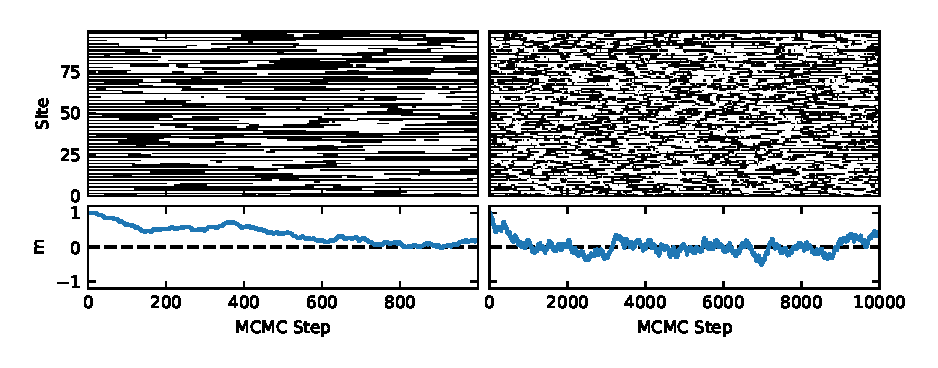
\includegraphics[width=1\textwidth,height=\textheight]{figure_code/fk_chapter/lsr/pdf_figs/raw_steps_single_flip}
\caption[{Comparison of different proposal distributions}]{Two Markov Chain Monte Carlo (MCMC) walks starting from the CDW state for a system with \(N = 100\) sites and 10,000 MCMC steps but at a temperature close to but above the ordered state (left column) and much higher than it (right column). In this simulation only a single spin can be flipped per step according to the Metropolis-Hastings Algorithm. The staggered magnetisation \(m = N^{-1} \sum_i (-1)^i \; S_i\) order parameter is plotted below. At both temperatures the thermal average of m is zero, while the initial state has m = 1. The higher temperature allows the MCMC to converge more quickly and to fluctuate about the mean with a shorter autocorrelation time. \(t = 1, \alpha = 1.25, T = {2.5,5}, J = U = 5\)}
\label{fig:raw_steps_single_flip}
\end{figure}
}

The classical Markov Chain Monte Carlo (MCMC) method which we discuss in the following allows us to solve our LRFK model efficiently, yielding unbiased estimates of thermal expectation values.

Since the spin configurations are classical, the LRFK Hamiltonian can be split into a classical spin part \(H_s\) and an operator valued part \(H_c\).

\[\begin{aligned}
H_s& = - \frac{U}{2}S_i + \sum_{i, j}^{N} J_{ij} S_i S_j \\
H_c& = \sum_i U S_i c^\dagger_{i}c_{i} -t(c^\dagger_{i}c_{i+1} + c^\dagger_{i+1}c_{i}) \end{aligned}\]

The partition function can then be written as a sum over spin configurations, \(\vec{S} = (S_0, S_1...S_{N-1})\):

\[\begin{aligned}
\mathcal{Z} = \mathrm{Tr} e^{-\beta H}= \sum_{\vec{S}} e^{-\beta H_s} \mathrm{Tr}_c e^{-\beta H_c} .\end{aligned}\]

The contribution of \(H_c\) to the grand canonical partition function can be obtained by performing the sum over eigenstate occupation numbers giving \(-\beta F_c[\vec{S}] = \sum_k \ln{(1 + e^{- \beta \epsilon_k})}\) where \({\epsilon_k[\vec{S}]}\) are the eigenvalues of the matrix representation of \(H_c\) determined through exact diagonalisation. This gives a partition function containing a classical energy which corresponds to the long-range interaction of the spins, and a free energy which corresponds to the quantum subsystem.

\[\begin{aligned}
\mathcal{Z} = \sum_{\vec{S}} e^{-\beta H_S[\vec{S}] - \beta F_c[\vec{S}]} = \sum_{\vec{S}} e^{-\beta E[\vec{S}]}\end{aligned}\]

\hypertarget{markov-chain-monte-carlo-and-emergent-disorder}{%
\subsection{Markov Chain Monte Carlo and Emergent Disorder}\label{markov-chain-monte-carlo-and-emergent-disorder}}

Classical MCMC defines a weighted random walk over the spin states \((\vec{S}_0, \vec{S}_1, \vec{S}_2, ...)\), such that the likelihood of visiting a particular state converges to its Boltzmann probability \(p(\vec{S}) = \mathcal{Z}^{-1} e^{-\beta E}\). Hence, any observable can be estimated as a mean over the states visited by the walk~\autocite{binderGuidePracticalWork1988,kerteszAdvancesComputerSimulation1998,wolffMonteCarloErrors2004},

\[\begin{aligned}
\label{eq:thermal_expectation}
\langle O \rangle & = \sum_{\vec{S}} p(\vec{S}) \langle O \rangle\\
                  & = \sum_{i = 0}^{M} \langle O\rangle \pm \mathcal{O}(M^{-\tfrac{1}{2}})
\end{aligned}\]

where the former sum runs over the entire state space while the later runs over all the state visited by a particular MCMC run.

\[\begin{aligned}
\langle O \rangle_{\vec{S}}& = \sum_{\nu} n_F(\epsilon_{\nu}) \langle O \rangle{\nu}
\end{aligned}\]

Where \(\nu\) runs over the eigenstates of \(H_c\) for a particular spin configuration and \(n_F(\epsilon) = \left(e^{-\beta\epsilon} + 1\right)^{-1}\) is the Fermi function.

The choice of the transition function for MCMC is under-determined as one only needs to satisfy a set of balance conditions for which there are many solutions~\autocite{kellyReversibilityStochasticNetworks1981}. Here, we incorporate a modification to the standard Metropolis-Hastings algorithm~\autocite{hastingsMonteCarloSampling1970} gleaned from Krauth~\autocite{krauthIntroductionMonteCarlo1998}.

The standard algorithm decomposes the transition probability into \(\mathcal{T}(a \to b) = p(a \to b)\mathcal{A}(a \to b)\). Here, \(p\) is the proposal distribution that we can directly sample from while \(\mathcal{A}\) is the acceptance probability. The standard Metropolis-Hastings choice is

\[\mathcal{A}(a \to b) = \min\left(1, \frac{p(b\to a)}{p(a\to b)} e^{-\beta \Delta E}\right)\;,\]

with \(\Delta E = E_b - E_a\). The walk then proceeds by sampling a state \(b\) from \(p\) and moving to \(b\) with probability \(\mathcal{A}(a \to b)\). The latter operation is typically implemented by performing a transition if a uniform random sample from the unit interval is less than \(\mathcal{A}(a \to b)\) and otherwise repeating the current state as the next step in the random walk. The proposal distribution is often symmetric so does not appear in \(\mathcal{A}\). Here, we flip a small number of sites in \(b\) at random to generate proposals, which is a symmetric proposal.

In our computations~\autocite{hodsonMCMCFKModel2021} the modification to this algorithm that we employ is based on the observation that the free energy of the FK system is composed of a classical part which is much quicker to compute than the quantum part. Hence, we can obtain a computational speed up by first considering the value of the classical energy difference \(\Delta H_s\) and rejecting the transition if the former is too high. We only compute the quantum energy difference \(\Delta F_c\) if the transition is accepted. We then perform a second rejection sampling step based upon it. This corresponds to two nested comparisons with the majority of the work only occurring if the first test passes. This modified scheme has the acceptance function \[\mathcal{A}(a \to b) = \min\left(1, e^{-\beta \Delta H_s}\right)\min\left(1, e^{-\beta \Delta F_c}\right)\;.\]

For the model parameters used, we find that with our new scheme the matrix diagonalisation is skipped around 30\% of the time at \(T = 2.5\) and up to 80\% at \(T = 1.5\). We observe that for \(N = 50\), the matrix diagonalisation, if it occurs, occupies around 60\% of the total computation time for a single step. This rises to 90\% at N = 300 and further increases for larger N. We therefore get the greatest speedup for large system sizes at low temperature where many prospective transitions are rejected at the classical stage and the matrix computation takes up the greatest fraction of the total computation time. The upshot is that we find a speedup of up to a factor of 10 at the cost of very little extra algorithmic complexity.

Our two-step method should be distinguished from the more common method for speeding up MCMC which is to add asymmetry to the proposal distribution to make it as similar as possible to \(\min\left(1, e^{-\beta \Delta E}\right)\). This reduces the number of rejected states, which brings the algorithm closer in efficiency to a direct sampling method. However it comes at the expense of requiring a way to directly sample from this complex distribution, a problem which MCMC was employed to solve in the first place. For example, recent work trains restricted Boltzmann machines (RBMs) to generate samples for the proposal distribution of the FK model~\autocite{huangAcceleratedMonteCarlo2017}. The RBMs are chosen as a parametrisation of the proposal distribution that can be efficiently sampled from while offering sufficient flexibility that they can be adjusted to match the target distribution. Our proposed method is considerably simpler and does not require training while still reaping some of the benefits of reduced computation.

\hypertarget{scaling}{%
\subsection{Scaling}\label{scaling}}

\hypertarget{fig:binder_cumulants}{%
\begin{figure}
\centering
\includegraphics[width=1\textwidth,height=\textheight]{figure_code/fk_chapter/binder_cumulants/binder_cumulants}
\caption[{Binder Cumulants}]{(Left) The order parameters, \(\langle m^2 \rangle\)(solid) and \(1 - f\) (dashed) describing the onset of the charge density wave phase of the long-range 1D Falicov model at low temperature with staggered magnetisation \(m = N^{-1} \sum_i (-1)^i S_i\) and fermionic order parameter \(f = 2 N^{-1}|\sum_i (-1)^i \; \langle c^\dagger_{i}c_{i}| \rangle\) . (Right) The crossing of the Binder cumulant, \(B = \langle m^4 \rangle / \langle m^2 \rangle^2\), with system size provides a diagnostic that the phase transition is not a finite size effect, it is used to estimate the critical lines shown in the phase diagram later. All plots use system sizes \(N = [10,20,30,50,70,110,160,250]\) and lines are coloured from \(N = 10\) in dark blue to \(N = 250\) in yellow. The parameter values \(U = 5,\;J = 5,\;\alpha = 1.25\) except where explicitly mentioned.}
\label{fig:binder_cumulants}
\end{figure}
}

To improve the scaling of finite size effects, we make the replacement \(|i - j|^{-\alpha} \rightarrow |f(i - j)|^{-\alpha}\), in both \(J_{ij}\) and \(\kappa\), where \(f(x) = \frac{N}{\pi}\sin \frac{\pi x}{N}\). \(f\) is smooth across the circular boundary and its effect effect diminished for larger systems~\autocite{fukuiOrderNClusterMonte2009}. We only consider even system sizes given that odd system sizes are not commensurate with a CDW state.

To identify critical points we use the the Binder cumulant \(U_B\) defined by

\[
U_B = 1 - \frac{\langle\mu_4\rangle}{3\langle\mu_2\rangle^2}
\]

where \(\mu_n = \langle(m - \langle m\rangle)^n\rangle\) are the central moments of the order parameter \(m = \sum_i (-1)^i (2n_i - 1) / N\). The Binder cumulant evaluated against temperature is a diagnostic for the existence of a phase transition. If multiple such curves are plotted for different system sizes, a crossing indicates the location of a critical point while the lines do not cross for systems that don't have a phase transition in the thermodynamic limit~\autocite{binderFiniteSizeScaling1981,musialMonteCarloSimulations2002}.

\hypertarget{fk-results}{%
\section{Results}\label{fk-results}}

Phase diagrams of the long-range 1D FK model. (a) The TJ plane at \(U = 5\): the CDW ordered phase is separated from a disordered Mott insulating (MI) phase by a critical temperature \(T_c\), linear in J. (b) The TU plane at \(J = 5\): the disordered phase is split into two: at large/small U there's a MI/Anderson phase characterised by the presence/absence of a gap at \(E=0\) in the single particle energy spectrum. \(U_c\) is independent of temperature. At \(U = 0\) the fermions are decoupled from the spins forming a simple Fermi gas. (c) The order parameters, \(\langle m^2 \rangle\)(solid) and \(1 - f\) (dashed) describing the onset of the {CDW} phase of the long-range 1D {FK} model at low temperature with staggered magnetisation \(m = N^{-1} \sum_i (-1)^i S_i\) and fermionic order parameter \(f = 2 N^{-1}|\sum_i (-1)^i \; \langle c^\dagger_{i}c_{i}| \rangle\) . (d) The crossing of the Binder cumulant, \(B = \langle m^4 \rangle / \langle m^2 \rangle^2\), with system size provides a diagnostic that the phase transition is not a finite size effect, it's used to estimate the critical lines shown in (a) and (b). All plots use system sizes \(N = [10,20,30,50,70,110,160,250]\) and lines are coloured from \(N = 10\) in dark blue to \(N = 250\) in yellow. The parameter values \(U = 5,\;J = 5,\;\alpha = 1.25\) except where explicitly varied.

\hypertarget{fig:binder}{%
\begin{figure}
\centering
\includegraphics[width=1\textwidth,height=\textheight]{figure_code/fk_chapter/binder.png}
\caption[{no title}]{Hello I am the figure caption!}
\label{fig:binder}
\end{figure}
}

\hypertarget{lrfk-results-phase-diagram}{%
\subsection{Phase Diagram}\label{lrfk-results-phase-diagram}}

Figs.~{[}\protect\hyperlink{fig:phase_diagram}{1}a{]} and {[}\protect\hyperlink{fig:phase_diagram}{1}b{]} show the phase diagram for constant \(U=5\) and constant \(J=5\), respectively. We determined the transition temperatures from the crossings of the Binder cumulants \(B_4 = \langle m^4 \rangle /\langle m^2 \rangle^2\)~\autocite{binderFiniteSizeScaling1981}. For a representative set of parameters, Fig.~{[}\protect\hyperlink{fig:phase_diagram}{1}c{]} shows the order parameter \(\rangle m \langle^2\). Fig.~{[}\protect\hyperlink{fig:phase_diagram}{1}d{]} shows the Binder cumulants, both as functions of system size and temperature. The crossings confirm that the system has a FTPT and that the ordered phase is not a finite size effect.

The CDW transition temperature is largely independent from the strength of the interaction \(U\). This demonstrates that the phase transition is driven by the long-range term \(J\) with little effect from the coupling to the fermions \(U\). The physics of the spin sector in our long-range FK model mimics that of the LRI model and is not significantly altered by the presence of the fermions, which shows that the long range tail expected from a basic fermion mediated RKKY interaction between the Ising spins is absent.

Our main interest concerns the additional structure of the fermionic sector in the high temperature phase. Following Ref.~\autocite{antipovInteractionTunedAndersonMott2016}, we can distinguish between the Mott and Anderson insulating phases. The former is characterised by a gapped DOS in the absence of a CDW. Thus, the opening of a gap for large \(U\) is distinct from the gap-opening induced by the translational symmetry breaking in the CDW state below \(T_c\), see also Fig.~{[}\protect\hyperlink{fig:band_opening}{3}a{]}. The Anderson phase is gapless but, as we explain below, shows localised fermionic eigenstates.

\hypertarget{localisation-properties}{%
\subsection{Localisation Properties}\label{localisation-properties}}

The MCMC formulation suggests viewing the spin configurations as a form of annealed binary disorder whose probability distribution is given by the Boltzmann weight \(e^{-\beta H_S[\vec{S}] - \beta F_c[\vec{S}]}\). This makes apparent the link to the study of disordered systems and Anderson localisation. While these systems are typically studied by defining the probability distribution for the quenched disorder potential externally, here we have a translation invariant system with disorder as a natural consequence of the Ising background field conserved under the dynamics.

In the limits of zero and infinite temperature, our model becomes a simple tight-binding model for the fermions. At zero temperature, the spin background is in one of the two translation invariant AFM ground states with two gapped fermionic CDW bands at energies \[E_{\pm} = \pm\sqrt{\frac{1}{4}U^2 + 2t^2(1 + \cos ka)^2}\;.\]

At infinite temperature, all the spin configurations become equally likely and the fermionic model reduces to one of binary uncorrelated disorder in which all eigenstates are Anderson localised~\autocite{abrahamsScalingTheoryLocalization1979}. An Anderson localised state centered around \(r_0\) has magnitude that drops exponentially over some localisation length \(\xi\) i.e \(|\psi(r)|^2 \sim \exp{-\abs{r - r_0}/\xi}\). Calculating \(\xi\) directly is numerically demanding. Therefore, we determine if a given state is localised via the energy-resolved IPR and the DOS defined as \[\begin{aligned}
\mathrm{DOS}(\vec{S}, \omega)& = N^{-1} \sum_{i} \delta(\epsilon_i - \omega)\\
\mathrm{IPR}(\vec{S}, \omega)& = \; N^{-1} \mathrm{DOS}(\vec{S}, \omega)^{-1} \sum_{i,j} \delta(\epsilon_i - \omega)\;\psi^{4}_{i,j}\end{aligned}\] where \(\epsilon_i\) and \(\psi_{i,j}\) are the \(i\)th energy level and \(j\)th element of the corresponding eigenfunction, both dependent on the background spin configuration \(\vec{S}\).

The scaling of the IPR with system size \[\mathrm{IPR} \propto N^{-\tau}\] depends on the localisation properties of states at that energy. For delocalised states, e.g.~Bloch waves, \(\tau\) is the physical dimension. For fully localised states \(\tau\) goes to zero in the thermodynamic limit. However, for special types of disorder such as binary disorder, the localisation lengths can be large comparable to the system size at hand, which can make it difficult to extract the correct scaling. An additional complication arises from the fact that the scaling exponent may display intermediate behaviours for correlated disorder and in the vicinity of a localisation-delocalisation transition~\autocite{kramerLocalizationTheoryExperiment1993,eversAndersonTransitions2008}. The thermal defects of the CDW phase lead to a binary disorder potential with a finite correlation length, which in principle could result in delocalized eigenstates.

The key question for our system is then: How is the \(T=0\) CDW phase with fully delocalized fermionic states connected to the fully localized phase at high temperatures?

\begin{figure}
\hypertarget{fig:indiv_IPR}{%
\centering
\includegraphics{pdf_figs/indiv_IPR}
\caption{Energy resolved DOS(\(\omega\)) and \(\tau\) (the scaling exponent of IPR(\(\omega\)) against system size \(N\)). The left column shows the Anderson phase \(U = 2\) at high \(T = 2.5\) and the CDW phase at low \(T = 1.5\) temperature. IPRs are evaluated for one of the in-gap states \(\omega_0/U = 0.057\) and the center of the band \(\omega_1\) \(U = 0.81\). The right column shows instead the Mott and CDW phases at \(U = 5\) with \(\omega_0/U = 0.24\) and \(\omega_1/U = 0.571\). For all the plots \(J = 5,\;\alpha = 1.25\) and the fits for \(\tau\) use system sizes greater than 60. The measured \(\tau_0,\tau_1\) for each figure are: (a) \((0.06\pm0.01, 0.02\pm0.01\) (b) \(0.04\pm0.02, 0.00\pm0.01\) (c) \(0.05\pm0.03, 0.30\pm0.03\) (d) \(0.06\pm0.04, 0.15\pm0.05\) We show later that the apparent scaling of the IPR with system size can be explained by the changing defect density with system size rather than due to delocalisation of the states.}\label{fig:indiv_IPR}
}
\end{figure}

\begin{figure}
\hypertarget{fig:band_opening}{%
\centering
\includegraphics{pdf_figs/gap_openingboth}
\caption{The DOS (a and c) and scaling exponent \(\tau\) (b and d) as a function of energy and temperature. (a) and (b) show the system transitioning from the CDW phase to the gapless Anderson insulating one at \(U=2\) while (c) and (d) show the CDW to gapped Mott phase transition at \(U=5\). Regions where the DOS is close to zero are shown a white. The scaling exponent \(\tau\) is obtained from fits to \(IPR(N) = A N^{-\lambda}\) for a range of system sizes. \(U = 5,\;J = 5,\;\alpha = 1.25\)}\label{fig:band_opening}
}
\end{figure}

\includegraphics[width=1\textwidth,height=\textheight]{../figure_code/fk_chapter/gap_opening_high_U} \includegraphics[width=1\textwidth,height=\textheight]{../figure_code/fk_chapter/gap_opening_low_U}

\begin{figure}
\hypertarget{fig:indiv_IPR_disorder}{%
\centering
\includegraphics{pdf_figs/indiv_IPR_disorder}
\caption{A comparison of the full FK model to a simple binary disorder model (DM) with a CDW wave background perturbed by uncorrelated defects at density \(0 < \rho < 1\) matched to the largest corresponding FK model. As in Fig~\protect\hyperlink{fig:indiv_IPR}{2}, the Energy resolved DOS(\(\omega\)) and \(\tau\) are shown. The DOSs match well and this data makes clear that the apparent scaling of IPR with system size is a finite size effect due to weak localisation~\autocite{antipovInteractionTunedAndersonMott2016}, hence all the states are indeed localised as one would expect in 1D. The disorder model \(\tau_0,\tau_1\) for each figure are: (a) \(0.01\pm0.05, -0.02\pm0.06\) (b) \(0.01\pm0.04, -0.01\pm0.04\) (c) \(0.05\pm0.06, 0.04\pm0.06\) (d) \(-0.03\pm0.06, 0.01\pm0.06\). The lines are fit on system sizes \(N > 400\)}\label{fig:indiv_IPR_disorder}
}
\end{figure}

Fig.~\protect\hyperlink{fig:indiv_IPR}{2} shows the DOS and \(\tau\), the scaling exponent of the IPR with system size, for a representative set of parameters covering all three phases. The DOS is symmetric about \(0\) because of the particle hole symmetry of the model. At high temperatures, all of the eigenstates are localised in both the Mott and Anderson phases (with \(\tau \leq 0.07\) for our system sizes). We also checked that the states are localised by direct inspection. Note that there are in-gap states for instance at \(\omega_0\), below the upper band which are localized and smoothly connected across the phase transition.

In the CDW phases at \(U=2\) and \(U=5\), we find for the states within the gapped CDW bands, e.g.~at \(\omega_1\), scaling exponents \(\tau = 0.30\pm0.03\) and \(\tau = 0.15\pm0.05\), respectively. This surprising finding suggests that the CDW bands are partially delocalised with multi-fractal behaviour of the wavefunctions~\autocite{eversAndersonTransitions2008}. This phenomenon would be unexpected in a 1D model as they generally do not support delocalisation in the presence of disorder except as the result of correlations in the emergent disorder potential~\autocite{croyAndersonLocalization1D2011,goldshteinPurePointSpectrum1977}. However, we later show by comparison to an uncorrelated Anderson model that these nonzero exponents are a finite size effect and the states are localised with a finite \(\xi\) similar to the system size. As a result, the IPR does not scale correctly until the system size has grown much larger than \(\xi\). Fig.~{[}\protect\hyperlink{fig:indiv_IPR_disorder}{4}{]} shows that the scaling of the IPR in the CDW phase does flatten out eventually.

Next, we use the DOS and the scaling exponent \(\tau\) to explore the localisation properties over the energy-temperature plane in Fig.~\protect\hyperlink{fig:band_opening}{3}. Gapped areas are shown in white, which highlights the distinction between the gapped Mott phase and the ungapped Anderson phase. In-gap states appear just below the critical point, smoothly filling the bandgap in the Anderson phase and forming islands in the Mott phase. As in the finite~\autocite{zondaGaplessRegimeCharge2019} and infinite dimensional~\autocite{hassanSpectralPropertiesChargedensitywave2007} cases, the in-gap states merge and are pushed to lower energy for decreasing U as the \(T=0\) CDW gap closes. Intuitively, the presence of in-gap states can be understood as a result of domain wall fluctuations away from the AFM ordered background. These domain walls act as local potentials for impurity-like bound states~\autocite{zondaGaplessRegimeCharge2019}.

In order to understand the localization properties we can compare the behaviour of our model with that of a simpler Anderson disorder model (DM) in which the spins are replaced by a CDW background with uncorrelated binary defect potentials, see Appendix~??. Fig.~{[}\protect\hyperlink{fig:indiv_IPR_disorder}{4}{]} compares the FK model to the disorder model at different system sizes, matching the defect densities of the disorder model to the FK model at \(N = 270\) above and below the CDW transition. We find very good, even quantitative, agreement between the FK and disorder models, which suggests that correlations in the spin sector do not play a significant role. As we can sample directly from the disorder model, rather than through MCMC, the samples are uncorrelated. Hence we can evaluate much larger system sizes with the disorder model which enables us to pin down the correct localisation effects. In particular, what appear to be delocalized states for small system sizes eventually turn out to be states with large localization length. The localization length diverges towards the ordered zero temperature CDW state. Overall, we see that the interplay of interactions, here manifest as a peculiar binary potential, and localization can be very intricate and the added advantage of our 1D model is that we can explore very large system sizes for a complete understanding.

\hypertarget{fk-conclusion}{%
\section{Discussion and Conclusion}\label{fk-conclusion}}

The FK model is one of the simplest non-trivial models of interacting fermions. We studied its thermodynamic and localisation properties brought down in dimensionality to 1D by adding a novel long-ranged coupling designed to stabilise the CDW phase present in dimension two and above. Our hybrid MCMC approach elucidates a disorder-free localization mechanism within our translationally invariant system. Further, we demonstrate a significant speedup over the naive method. We show that our long-range FK in 1D retains much of the rich phase diagram of its higher dimensional cousins. Careful scaling analysis indicates that all the single particle eigenstates eventually localise at nonzero temperature albeit only for very large system sizes of several thousand.

Our work raises a number of interesting questions for future research. A straightforward but numerically challenging problem is to pin down the model's behaviour closer to the critical point where correlations in the spin sector would become significant. Would this modify the localisation behaviour? Similar to other soluble models of disorder-free localisation, we expect intriguing out-of equilibrium physics, for example slow entanglement dynamics akin to more generic interacting systems~\autocite{hartLogarithmicEntanglementGrowth2020}. One could also investigate whether the rich ground state phenomenology of the FK model as a function of filling~\autocite{gruberGroundStatesSpinless1990} such as the devil's staircase~\autocite{michelettiCompleteDevilTextquotesingles1997} could be stabilised at finite temperature. In a broader context, we envisage that long-range interactions can also be used to gain a deeper understanding of the temperature evolution of topological phases. One example would be a long-ranged FK version of the celebrated Su-Schrieffer-Heeger model where one could explore the interplay of topological bound states and thermal domain wall defects. Finally, the rich physics of our model should be realizable in systems with long-range interactions, such as trapped ion quantum simulators, where one can also explore the fully interacting regime with a dynamical background field.

\textbf{UNCORRELATED DISORDER MODEL}

The disorder model referred to in the main text is defined by replacing the spin degree of freedom in the FK model \(S_i = \pm \tfrac{1}{2}\) with a disorder potential \(d_i = \pm \tfrac{1}{2}\) controlled by a defect density \(\rho\) such that \(d_i = -\tfrac{1}{2}\) with probability \(\rho/2\) and \(d_i = \tfrac{1}{2}\) otherwise. \(\rho/2\) is used rather than \(\rho\) so that the disorder potential takes on the zero temperature CDW ground state at \(\rho = 0\) and becomes a random choice over spin states at \(\rho = 1\) i.e the infinite temperature limit. ~ \[\begin{aligned}
H_{\mathrm{DM}} = & \;U \sum_{i} (-1)^i \; d_i \;(c^\dag_{i}c_{i} - \tfrac{1}{2}) \\
& -\;t \sum_{i} c^\dag_{i}c_{i+1} + c^\dag_{i+1}c_{i} \nonumber\end{aligned}\]

Could look at doping the mott insulating phase, see results like~\autocite{caiVisualizingEvolutionMott2016}

\begin{Shaded}
\begin{Highlighting}[]

\end{Highlighting}
\end{Shaded}

\printbibliography[heading=subbibintoc]
\end{refsection}

\hypertarget{chap:4-the-amorphous-kitaev-model}{\chapter{The Amorphous Kitaev Honeycomb Model}}
\backgroundsetup{scale = 1, angle = 0, opacity = 1,
  contents = {\includegraphics[width=297mm, height=297mm]{figure_code/amk_chapter_background_mockup.pdf}}}
\BgThispage
\begin{refsection}
\hypertarget{ak-contributions}{%
\subsubsection{Contributions}\label{ak-contributions}}

The material in this chapter expands on work presented in

~\autocite{cassellaExactChiralAmorphous2022} Cassella, G., D'Ornellas, P., Hodson, T., Natori, W. M., \& Knolle, J. (2022). An exact chiral amorphous spin liquid. \emph{arXiv preprint arXiv:2208.08246.}

All the code is available online as a Python package called Koala~\autocite{hodsonKoalaKitaevAmorphous2022}.

This was a joint project of Gino, Peru and me with advice and guidance from Willian and Johannes, all authors of the above. The project grew out of an interest the three of us had in studying amorphous systems, coupled with Johannes' expertise on the Kitaev model. The idea to use Voronoi partitions came from ref.~\autocite{marsalTopologicalWeaireThorpe2020} and Gino did the implementation of this. The idea and implementation of the edge colouring using SAT solvers and the mapping from flux sector to bond sector using A* search were both entirely my work. Peru produced the numerical evidence for the ground state and implemented the local markers. Gino and I did much of the rest of the programming for Koala collaboratively, often pair programming, this included the phase diagram, edge mode and finite temperature analyses as well as the derivation of the projector in the amorphous case.

\hypertarget{ak-summary}{%
\subsubsection{Chapter Summary}\label{ak-summary}}

In this chapter, I will first define the amorphous Kitaev (AK) model and discuss the construction of amorphous lattices. Second, in the~\protect\hyperlink{amk-methods}{methods} section I will discuss the details of voronisation and graph colouring. Finally, I will present and interpret the~\protect\hyperlink{amk-results}{results} obtained.

From its introduction it was known that the Kitaev Honeycomb (KH) model is solvable on any trivalent lattice. Consequently, it has been generalised to many such lattices~\autocite{eschmannThermodynamicClassificationThreedimensional2020,Yao2009,eschmann2019thermodynamics,Peri2020} but so far none that entirely lack translation symmetry. Here we will do just that.

Amorphous lattices are characterised by local constraints but no long-range order. They arise, for instance, in amorphous semiconductors~like silicon and germanium~\autocite{Yonezawa1983,zallen2008physics}. Recent work has shown that topological insulating (TI) phases, characterised by protected edge states and topological bulk invariants, can exist in amorphous systems~\autocite{mitchellAmorphousTopologicalInsulators2018,agarwala2019topological,marsalTopologicalWeaireThorpeModels2020,costa2019toward,agarwala2020higher,spring2021amorphous,corbae2019evidence}. TI phases, however, arise in non-interacting systems. In this context, we might ask whether Quantum Spin Liquid (QSL) systems and the Kitaev Honeycomb (KH) model, in particular, could be realised on amorphous lattices. The phases of the KH model have many similarities with TIs but differ in that the KH model is an interacting system. In general, research on amorphous electronic systems has been focused mainly on non-interacting systems with the exception of amorphous superconductivity~\autocite{buckel1954einfluss,mcmillan1981electron,meisel1981eliashberg,bergmann1976amorphous,mannaNoncrystallineTopologicalSuperconductors2022} or very recent work looking to understand the effect of strong electron repulsion in TIs~\autocite{kim2022fractionalization}.

The KH model is a magnetic system. Magnetism in amorphous systems has been investigated since the 1960s, mostly through the adaptation of theoretical tools developed for disordered systems~\autocite{aharony1975critical,Petrakovski1981,kaneyoshi1992introduction,Kaneyoshi2018}. This is not always ideal, we have already seen that the topological disorder of amorphous lattices can be qualitatively different from standard bond or site disorder, especially in 2D~\autocite{barghathiPhaseTransitionsRandom2014,schrauthViolationHarrisBarghathiVojtaCriterion2018}. Research focused on classical Heisenberg and Ising models has accounted for the observed behaviour of ferromagnetism, disordered antiferromagnetism and widely observed spin glass behaviour~\autocite{coey1978amorphous}. However, the role of the spin-anisotropic interactions and quantum effects that we see in the KH model has not been addressed in amorphous magnets. It is an open question whether frustrated magnetic interactions on amorphous lattices can give rise to genuine quantum phases such as QSLs~\autocite{Anderson1973,Knolle2019,Savary2016,Lacroix2011}. This chapter will answer that question by demonstrating that the Kitaev model on amorphous lattices leads to a kind of QSL called a chiral spin liquid.

In this section, I will discuss how to generalise the KH to an amorphous lattice. The \protect\hyperlink{amk-methods}{methods section} discusses how to generate amorphous lattices using Voronoi partitions of the plane~\autocite{mitchellAmorphousTopologicalInsulators2018,marsalTopologicalWeaireThorpeModels2020}, colour them using a SAT solver and how to map back and forth between gauge field configurations and flux configurations. In the \protect\hyperlink{amk-results}{results section}, I will show extensive numerical evidence that the AK model follows the simple generalisation to Lieb's theorem~\autocite{lieb_flux_1994} found by other works~\autocite{eschmannThermodynamicClassificationThreedimensional2020,Yao2009,eschmann2019thermodynamics,Peri2020}. I then map out the phase diagram of the AK model and show that the chiral phase around the symmetric point (\(J_x = J_y = J_z\)) is gapped and non-Abelian. We use a quantised local Chern number \(\nu\)~\autocite{peru_preprint,mitchellAmorphousTopologicalInsulators2018} as well as the presence of protected chiral Majorana edge modes to determine this. Finally, I look at the role of finite temperature fluctuations and show that the proliferation of flux excitations leads to an Anderson transition, similar to that of the Falicov-Kimball model, to a thermal metal phase~\autocite{Laumann2012,lahtinenTopologicalLiquidNucleation2012,selfThermallyInducedMetallic2019}. Finally, I consider possible physical realisations of the AK model and other generalisations.

\hypertarget{amk-Model}{%
\section{The Model}\label{amk-Model}}

\hypertarget{fig:amk-zoom}{%
\begin{figure}
\centering
\includegraphics[width=1\textwidth,height=\textheight]{figure_code/amk_chapter/intro/amk_zoom/amk_zoom_by_hand}
\caption[{The Kitaev Honeycomb Model}]{\textbf{(a)} The standard Kitaev model is defined on a honeycomb lattice. The special feature of the honeycomb lattice that makes the model solvable is that each vertex is joined by exactly three bonds, i.e., the lattice is trivalent. One of three labels is assigned to each \textbf{(b)}. We represent the antisymmetric gauge degree of freedom \(u_{jk} = \pm 1\) with arrows that point in the direction \(u_{jk} = +1\) \textbf{(c)}. The Majorana transformation can be visualised as breaking each spin into four Majoranas which then pair along the bonds. Pairs of \(b_i^x,\;b_i^y\) and \(b_i^z\) Majoranas become part of the classical \(\mathbb{Z}_2\) gauge field \(u_{ij}\). This leaves a single Majorana \(c_i\) per site.}
\label{fig:amk-zoom}
\end{figure}
}

The KH model is solvable on any lattice which satisfies two properties: it must be trivalent and it must three-edge-colourable. The first property means every vertex must have three edges attached to it~\autocite{kitaevAnyonsExactlySolved2006,Nussinov2009}. 2D Voronoi lattices are a well-studied class of amorphous trivalent lattices~\autocite{mitchellAmorphousTopologicalInsulators2018,florescu_designer_2009,marsalTopologicalWeaireThorpeModels2020}. Given a set of seed points, the Voronoi partition divides the plane into basins, based on which seed point is closest by some metric, usually the euclidean metric. The basins of each seed point form the plaquettes of the resulting lattices, while the boundaries become the edges. The Voronoi partition exists in arbitrary dimension \(d\) and produces lattices with degree \(d+1\) except for degenerate cases with measure zero~\autocite{voronoiNouvellesApplicationsParamètres1908,watsonComputingNdimensionalDelaunay1981}. Voronoi lattices in 2D are trivalent so lend themselves naturally to the Kitaev model.

Other methods of lattice generation exist. One can connect randomly placed sites based on proximity~\autocite{agarwala2019topological} or create simplices from random sites~\autocite{christRandomLatticeField1982}. However, these methods do not present a natural way to restrict the vertex degree to a constant. The most unbiased way to select trivalent graphs would be to sample uniformly from the space of possible trivalent graphs. There has been some work on how to do this using a Markov Chain Monte Carlo approach~\autocite{alyamiUniformSamplingDirected2016}. However, it does not guarantee that the resulting graph is planar, which is necessary to be able to three-edge-colour the lattice, our second constraint.

The second constraint, three-edge-colourability, requires that we must be able to assign labels to each bond \(\{x,y,z\}\) such that no two edges with the same label meet at a vertex. Such an assignment is known as a three-edge-colouring. For translation invariant models we need only find a solution for the unit cell. This problem is usually small enough that this can be done by hand or using symmetry. For amorphous lattices, the difficulty is that, to the best of my knowledge, the problem of edge-colouring these lattices in general is in NP. To find colourings in practice, we will employ a standard method from the computer science literature for finding solutions of NP problems called a SAT solver, this is discussed in more detail in the \protect\hyperlink{amk-methods}{methods secton}.

We find that for large lattices there are many valid colourings. In the isotropic case \(J^\alpha = 1\) the colouring has no physical significance as the definition of the four Majoranas at a site is arbitrary. In the anisotropic case this symmetry is broken at the local level but we nevertheless expect the lattices to exhibit a self-averaging behaviour in larger systems such that the choice of colouring doesn't matter.

\hypertarget{fig:state_decomposition_animated}{%
\begin{figure}
\centering
\includegraphics[width=1\textwidth,height=\textheight]{figure_code/amk_chapter/intro/state_decomposition_animated/state_decomposition_animated}
\caption[{State Decomposition}]{(Bond Sector) A state in the bond sector is specified by assigning \(\pm 1\) to each edge of the lattice. However, this description has a substantial gauge degeneracy. To remove it, we decompose each state into the product of three kinds of objects: (Flux Sector) The main physically relevant quantities. Only a small number of bonds need to be flipped (compared to some arbitrary fixed reference) to reconstruct the flux sector. Here, the edges are chosen from a spanning tree of the dual lattice, so there are no loops. (Gauge Field) The `loopiness' of the bond sector is in this part. This is a network of loops that can always be written as a product of the gauge operators \(D_j\). (Topological Sector) Finally, there are two loops that have no effect on the vortex sector, nor can they be constructed from gauge symmetries \(D_j\). These can be thought of as two fluxes \(\Phi_{x/y}\) that thread through the major and minor axes of the torus. Measuring \(\Phi_{x/y}\) amounts to constructing Wilson loops around the axes of the torus. We can flip the value of \(\Phi_{x}\) by transporting a vortex pair around the torus in the \(y\) direction, as shown here. In each of the three figures on the right, black bonds correspond to those that must be flipped, while red line are those same edges on the dual lattice. Composing the three objects together gives back the original bond sector on the left. \href{http://thomashodson.com/assets/thesis/amk_chapter/intro/state_decomposition_animated/state_decomposition_animated.gif}{ Animated version online.}}
\label{fig:state_decomposition_animated}
\end{figure}
}

On a lattice with the above properties, the solution for the KH model laid out in~\protect\hyperlink{bg-hkm-model}{section 2.2} remains applicable to our AK model. See \cref{fig:amk-zoom} for an example lattice generated by our method. The main differences are twofold. Firstly, the lattices are no longer bipartite in general and therefore contain plaquettes with an odd number of sides which enclose flux \(\pm i\). This leads the AK model to have a ground state with spontaneously broken chiral symmetry~\autocite{Chua2011,yaoExactChiralSpin2007,ChuaPRB2011,Fiete2012,Natori2016,Wu2009,Peri2020,WangHaoranPRB2021}. This is analogous to the behaviour of the original Kitaev model in response to a magnetic field. One ground state is related to the other by globally inverting the imaginary \(\phi_i\) fluxes~\autocite{yaoExactChiralSpin2007}. Secondly, as the model is no longer translationally invariant, Lieb's theorem for the ground state flux sector no longer applies. However, as discussed in the background, a simple generalisation of Lieb's theorem has been shown numerically to be applicable to many generalised Kitaev models~\autocite{eschmannThermodynamicClassificationThreedimensional2020,Yao2009,eschmann2019thermodynamics,Peri2020}. This generalisation states that the ground state flux configuration depends on the number of sides of each plaquette as

\begin{equation}\protect\hypertarget{eq:gs-flux-sector}{}{\phi = -(\pm i)^{n_{\mathrm{sides}}},}\label{eq:gs-flux-sector}\end{equation}

with a twofold global chiral degeneracy (picking either \(+i\) or \(-i\) in \cref{eq:gs-flux-sector}).

To verify numerically that Lieb's theorem generalises to the AK model, the obvious approach would be via exhaustive checking of flux configurations. However, this is problematic because the number of states to check scales exponentially with system size. We side-step this by gluing together two methods, we first work with lattices small enough that we can fully enumerate their flux sectors but tile them to reduce finite size effects. We then show that the effect of tiling scales away with system size.

\hypertarget{fig:majorana_bound_states_animated}{%
\begin{figure}
\centering
\includegraphics[width=1\textwidth,height=\textheight]{figure_code/amk_chapter/intro/majorana_bound_states_animated/majorana_bound_states_animated}
\caption[{Majorana Bound States}]{(Left) A large amorphous lattice in the ground state save for a single pair of vortices shown in red, separated by the string of bonds that we flipped to create them. (Right) The density of the lowest energy Majorana state in this vortex sector. These Majorana states are bound to the vortices. They `dress' the vortices to create a composite object.}
\label{fig:majorana_bound_states_animated}
\end{figure}
}

In order to evaluate the Chern marker later, we need a way to evaluate the model on open boundary conditions. Simply removing bonds from the lattice leaves behind unpaired \(b^\alpha\) operators that must be paired in some way to arrive at fermionic modes. To fix a pairing, we always start from a lattice defined on the torus and generate a lattice with open boundary conditions by defining the bond coupling \(J^{\alpha}_{ij} = 0\) for sites joined by bonds \((i,j)\) that we want to remove. This creates fermionic zero modes \(u_{ij}\) associated with these cut bonds which we set to 1 when calculating the projector. Alternatively, since all the fermionic zero modes are degenerate anyway, an arbitrary pairing of the unpaired \(b^\alpha\) operators can be performed.

\hypertarget{the-euler-equation}{%
\subsection{The Euler Equation}\label{the-euler-equation}}

Euler's equation provides a convenient way to understand how the states of the AK model factorise into flux sectors, gauge sectors and topological sectors as in \cref{fig:state_decomposition_animated}. The Euler equation states that if we embed a lattice with \(B\) bonds, \(P\) plaquettes and \(V\) vertices onto a closed surface of genus \(g\), (\(0\) for the sphere, \(1\) for the torus) then

\[B = P + V + 2 - 2g.\]

For the case of the torus where \(g = 1\), we can rearrange this and exponentiate it to read:

\[2^B = 2^{P-1}\cdot 2^{V-1} \cdot 2^2.\]

There are \(2^B\) configurations of the bond variables \(\{u_{ij}\}\). Each of these configurations can be uniquely decomposed into a flux sector, a gauge sector and a topological sector, see \cref{fig:state_decomposition_animated}. Each of the \(P\) plaquette operators \(\phi_i\) takes two values but vortices are created in pairs so there are \(2^{P-1}\) vortex sectors in total. There are \(2^{V-1}\) gauge symmetries formed from the \(V\) symmetry operators \(D_i\) because \(\prod_{j} D_j = \mathbb{I}\) is enforced by the projector. Finally, the two topological fluxes \(\Phi_x\) and \(\Phi_y\) account for the last factor of \(2^2\).

In a trivalent lattice, there are three bonds for every 2 vertices. Substituting \(3V = 2B\) into Euler's equation tells us that any trivalent lattice on the torus with \(N\) plaquettes has \(2N\) vertices and \(3N\) bonds. Since each bond is part of two plaquettes this implies that the mean number of sides of a plaquette is exactly six and that odd sided plaquettes must come in pairs.

\hypertarget{amk-methods}{%
\section{Methods}\label{amk-methods}}

This section describes the novel methods we developed to simulate the AK model including lattice generation, bond colouring and the inverse mapping between flux sector and gauge sector. Implementations are available online as a Python package called Koala (Kitaev On Amorphous LAttices)~\autocite{hodsonKoalaKitaevAmorphous2022}. All results and figures herein were generated with Koala.

\hypertarget{voronisation}{%
\subsection{Voronisation}\label{voronisation}}

\hypertarget{fig:lattice_construction_animated}{%
\begin{figure}
\centering
\includegraphics[width=1\textwidth,height=\textheight]{figure_code/amk_chapter/lattice_construction_animated/lattice_construction_animated}
\caption[{Lattice Construction}]{(Left) Lattice construction begins with the Voronoi partition of the plane with respect to a set of seed points (black points) sampled uniformly from \(\mathbb{R}^2\). (Center) However, we want the Voronoi partition of the torus, so we tile the seed points into a three by three grid. The boundaries of each tile are shown in light grey. (Right) Finally, we identify edges corresponding to each other across the boundaries to produce a graph on the torus. \href{http://thomashodson.com/assets/thesis/amk_chapter/lattice_construction_animated/lattice_construction_animated.gif}{ Animated version online.}}
\label{fig:lattice_construction_animated}
\end{figure}
}

The lattices we use are Voronoi partitions of the torus~\autocite{mitchellAmorphousTopologicalInsulators2018,marsalTopologicalWeaireThorpeModels2020,florescu_designer_2009}. We start by sampling \emph{seed points} uniformly (or otherwise) on the torus. As most off the shelf routines for computing Voronoi partitions are defined on the plane rather than the torus, we tile our seed points into a \(3\times3\) pr \(5\times5\) grid before calling a standard Voronoi routine~\autocite{barberQuickhullAlgorithmConvex1996} from the python package Scipy~\autocite{virtanenSciPyFundamentalAlgorithms2020}. Finally, we undo the tiling to the grid by identifying edges in the tiled lattice which are identical, yielding a trivalent lattice on the torus. We encode our lattices with edge lists \([(i,j), (j,k)\ldots]\) and an additional vector \((\{-1,0,+1\}, \{-1,0,+1\})\) for each edge that encodes the sense in which it crosses the periodic boundary conditions, equivalent to how the edge leaves the unit cell were the system to tile the plane, see \protect\hyperlink{app-lattice-generation}{appendix A.3} for more detail.

The graph generated by a Voronoi partition of a 2D surface is always planar. This means that no edges cross each other when the graph is embedded into the plane. It is also trivalent in that every vertex is connected to exactly three edges~\autocite{voronoiNouvellesApplicationsParamètres1908,watsonComputingNdimensionalDelaunay1981}.

\hypertarget{colouring-the-bonds}{%
\subsection{Colouring the Bonds}\label{colouring-the-bonds}}

\hypertarget{fig:multiple_colourings}{%
\begin{figure}
\centering
\includegraphics[width=1\textwidth,height=\textheight]{figure_code/amk_chapter/multiple_colourings/multiple_colourings}
\caption[{Colourings of an Amorphous Lattice}]{Different valid three-edge-colourings of an amorphous lattice. Colors that differ from the leftmost panel are highlighted in the other panels.}
\label{fig:multiple_colourings}
\end{figure}
}

To be solvable the AK model requires that each edge in the lattice be assigned a label \(x\), \(y\) or \(z\), such that each vertex has exactly one edge of each type connected to it. This problem must be distinguished from that considered by the famous four-colour theorem~\autocite{appelEveryPlanarMap1989}. The four-colour theorem is concerned with assigning colours to the \textbf{vertices} of planar graphs, such that no vertices that share an edge have the same colour. Here we are instead concerned with finding an edge colouring.

For a graph of maximum degree \(\Delta\), \(\Delta + 1\) colours are always enough to edge-colour it. An \(\mathcal{O}(mn)\) algorithm exists to do this for a graph with \(m\) edges and \(n\) vertices~\autocite{gEstimateChromaticClass1964}. Restricting ourselves to graphs with \(\Delta = 3\), these graphs are known as cubic graphs. Cubic graphs can be four-edge-coloured in linear time~\autocite{skulrattanakulchai4edgecoloringGraphsMaximum2002}. However we need a three-edge-colouring of our cubic graphs, which turns out to be more difficult. Cubic, planar, \emph{bridgeless} graphs can be three-edge-coloured if and only if they can be four-face-coloured~\autocite{tait1880remarks}. Bridges are edges that connect otherwise disconnected components. An \(\mathcal{O}(n^2)\) algorithm exists for these~\autocite{robertson1996efficiently}. However, it is not clear whether this extends to cubic, \textbf{toroidal} bridgeless graphs.

A four-face-colouring is equivalent to a four-vertex-colouring of the dual graph, see \protect\hyperlink{app-lattice-generation}{appendix A.3}. So if we could find a four-vertex-colouring of the dual graph we would be done. However vertex-colouring a toroidal graph may require up to seven colours~\autocite{heawoodMapColouringTheorems}! The complete graph of seven vertices \(K_7\) is a good example of a toroidal graph that requires seven colours.

Luckily, some problems are harder in theory than in practice. Three-edge-colouring cubic toroidal graphs appears to be one of those things. To find colourings, we use a Boolean Satisfiability Solver or SAT solver. A SAT problem is a set of statements about a set of boolean variables, such as ``\(x_1\) or not \(x_3\) is true''. A solution to a SAT problem is a assignment \(x_i \in {0,1}\) that satisfies all the statements~\autocite{Karp1972}. General purpose, high performance programs for solving SAT problems have been an area of active research for decades~\autocite{alounehComprehensiveStudyAnalysis2019}. Such programs are useful because, by the Cook-Levin theorem, any NP problem can be encoded (in polynomial time) as an instance of a SAT problem . This property is what makes SAT one of the subset of NP problems called NP-Complete~\autocite{cookComplexityTheoremprovingProcedures1971,levin1973universal}. Thus, it is a relatively standard technique in the computer science community to solve NP problems by first transforming them to SAT instances and then using an off the shelf SAT solver. The output of this can then be mapped back to the original problem domain.

Whether graph colouring problems are in NP or P seems to depend delicately on the class of graphs considered, the maximum degree and the number of colours used. Since we I didn't know of any better algorithm for the problem at hand using a SAT solver appeared to be a reasonable first method to try and it turns out to be fast enough in practice that it is by no means to rate limiting step for solving instances of our model. In \protect\hyperlink{app-lattice-generation}{appendix A.3} I detail the specifics of how I mapped edge-colouring problems to SAT instances and show a breakdown of where the computational effort is spent, the majority being on diagonalisation.

\hypertarget{mapping-between-flux-sectors-and-bond-sectors}{%
\subsection{Mapping between flux sectors and bond sectors}\label{mapping-between-flux-sectors-and-bond-sectors}}

\hypertarget{fig:flux_finding}{%
\begin{figure}
\centering
\includegraphics[width=1\textwidth,height=\textheight]{figure_code/amk_chapter/flux_finding/flux_finding}
\caption[{Finding Bond Sectors from Flux Sectors}]{(Left) The ground state flux sector and bond sector for an amorphous lattice. Bond arrows indicate the direction in which \(u_{jk} = +1\). Plaquettes are coloured blue when \(\hat{\phi}_i = -1\) (\(-i\)) for even/odd plaquettes and orange when \(\hat{\phi}_i = +1\) (\(+i\)) for even/odd plaquettes. (Centre) To transform this to the target flux sector (all \(+1\)/\(+i\)), we first flip any \(u_{jk}\) that are between two fluxes. This leaves a set of isolated fluxes that must be annihilated. Then, these are paired up as indicated by the black lines. (Right) A* search is used to find paths (coloured plaquettes) on the dual lattice between each pair of fluxes and the corresponding \(u_{jk}\) (shown in black) are flipped. One flux will remain because the starting and target flux sectors differed by an odd number of fluxes.}
\label{fig:flux_finding}
\end{figure}
}

In the AK model, going from the bond sector to flux sector is done simply from the definition of the fluxes

\[ \phi_i = \prod_{(j,k) \; \in \; \partial \phi_i} i u_{jk}.\]

The reverse, constructing the bond sector \(\{u_{jk}\}\) that corresponds to a particular flux sector \(\{\{\Phi_i\}\) is not so trivial. The algorithm, shown visually in \cref{fig:flux_finding} is this:

\begin{enumerate}
\def\labelenumi{\arabic{enumi}.}
\item
  Fix the gauge by choosing some arbitrary \(u_{jk}\) configuration. In practice, we use \(u_{jk} = +1\). This chooses an arbitrary one of the four topological sectors.
\item
  Compute the current flux configuration and how it differs from the target one. Consider any plaquette that differs from the target as a defect.
\item
  Find any adjacent pairs of defects and flip the \(u_jk\) between them. This leaves a set of isolated defects.
\item
  Pair the defects up using a greedy algorithm and compute paths along the dual lattice between each pair of plaquettes using A*. Flipping the corresponding set of bonds transports one flux to the other and annihilates both.
\end{enumerate}

\hypertarget{sec:AMK-Results}{%
\section{Results}\label{sec:AMK-Results}}

\hypertarget{the-ground-state-flux-sector}{%
\subsection{The Ground State Flux Sector}\label{the-ground-state-flux-sector}}

Here I will discuss the numerical evidence that our guess for the ground state flux sector is correct. We will do this by enumerating all the flux sectors of many separate system realisations. However there are some issues we will need to address to make this argument work.

We have two seemingly irreconcilable problems. Finite size effects have a large energetic contribution for small systems~\autocite{kitaevAnyonsExactlySolved2006} so we would like to perform our analysis for very large lattices. However for an amorphous system with \(N\) plaquettes, \(2N\) edges and \(3N\) vertices we have \(2^{N-1}\) flux sectors to check and diagonalisation scales with \(\mathcal{0}(N^3)\). That exponential scaling makes it infeasible to work with lattices much larger than \(16\) plaquettes.

To get around this we instead look at periodic systems with amorphous unit cells. For a similarly sized periodic system with \(A\) unit cells and \(B\) plaquettes in each unit cell where \(N \sim AB\) things get much better. We can use Bloch's theorem to diagonalise this system in about \(\mathcal{0}(A B^3)\) operations, and more importantly there are only \(2^{B-1}\) flux sectors to check.

We fully enumerated the flux sectors of \textasciitilde25,000 periodic systems with disordered unit cells of up to \(B = 16\) plaquettes and \(A = 100\) unit cells.

However, showing that our guess is correct for periodic systems with disordered unit cells is not quite convincing on its own. We have effectively removed longer-range disorder from our lattices.

The second part of the argument is to show that the energetic effect of introducing periodicity scales away as we go to larger system sizes and has already diminished to a small enough value at 16 plaquettes, which is indeed what we find.

From this we argue that the results for small periodic systems generalise to large amorphous systems. We perform this analysis for both the isotropic point (\(J^\alpha = 1\)), as well as in the toric code phase (\(J^x = J^y = 0.25, J^z = 1\)).

In the isotropic case (\(J^\alpha = 1\)), our conjecture correctly predicted the ground state flux sector for all of the lattices we tested.

For the toric code phase (\(J^x, J^y = 0.25, J^z = 1\)) all but around (\(\sim 0.5 \%\)) lattices had ground states conforming to our conjecture. In these cases, the energy difference between the true ground state and our prediction was on the order of \(10^{-6} J\). It is unclear whether this is a finite size effect or something else.

\hypertarget{spontaneous-chiral-symmetry-breaking}{%
\subsection{Spontaneous Chiral Symmetry Breaking}\label{spontaneous-chiral-symmetry-breaking}}

The spin Kitaev Hamiltonian is real and therefore has time reversal symmetry (TRS). However, the flux \(\phi_p\) through any plaquette with an odd number of sides has imaginary eigenvalues \(\pm i\). The ground state sector induces a relatively regular pattern for the imaginary fluxes with only a global two-fold chiral degeneracy.

Thus, states with a fixed flux sector spontaneously break time reversal symmetry. This was first described by Yao and Kivelson~for a translation invariant Kitaev model with odd sided plaquettes~\autocite{Yao2011}.

So we have flux sectors that come in degenerate pairs, where time reversal is equivalent to inverting the flux through every odd plaquette, a general feature for lattices with odd plaquettes~\autocite{yaoExactChiralSpin2007,Peri2020}. This spontaneously broken symmetry avoids the need to explicitly break TRS with a magnetic field term as is done in the original honeycomb model.

\hypertarget{ground-state-phase-diagram}{%
\subsection{Ground State Phase Diagram}\label{ground-state-phase-diagram}}

As previously discussed, the standard Honeycomb model has a Abelian, gapped phase in the anisotropic region (the A phase) and is gapless in the isotropic region. The introduction of a magnetic field breaks the chiral symmetry, leading to the isotropic region becoming a gapped, non-Abelian phase, the B phase.

We set the energy scale by requiring that \(J_x + J_y + J_z = 1\), this restricts the 3D phase space down to an equilateral triangle that is convenient for diagrams. Imagine the cube defined by \(J_\alpha \in [0,1]\) being cut by the plane \(J_x + J_y + J_z = 1\), we plot the projection of that plane in diagrams like \cref{fig:phase_diagram}.

Similar to the Kitaev Honeycomb model with a magnetic field, we find that the amorphous model is only gapless along critical lines, see \cref{fig:phase_diagram} (Left).

Interestingly, the gap closing exists in only one of the four topological sectors, though this is certainly a finite size effect as the sectors must become degenerate in the thermodynamic limit. Nevertheless this could be a useful way to define the (0, 0) topological flux sector for the amorphous model.

In the honeycomb model, the phase boundaries are located on the straight lines \(|J^x| = |J^y| + |J^x|\) and permutations of \(x,y,z\), shown as dotted line on \textasciitilde{}\ref{fig:phase_diagram} (Right). We find that on the amorphous lattice these boundaries exhibit an inward curvature, similar to honeycomb Kitaev models with flux~\autocite{Nasu_Thermal_2015} or bond~\autocite{knolle_dynamics_2016} disorder.

\hypertarget{fig:phase_diagram}{%
\begin{figure}
\centering
\includegraphics[width=1\textwidth,height=\textheight]{figure_code/amk_chapter/results/phase_diagram/phase_diagram}
\caption[{The Ground State Phase Diagram}]{(Center) We choose an energy scale for the Hamiltonian by setting \(J_x + J_y + J_z = 1\). This intersects a plane with the unit cube spanned by \(J_\alpha \in [0,1]\), giving a triangle with corners \((1,0,0), (0,1,0), (0,0,1)\). To compute critical lines efficiently in this space we evaluate the order parameter of interest along rays shooting from the corners. The ray highlighted in red defines the values of J used for the left figure. (Left) The fermion gap as a function of J for an amorphous system with 20 plaquettes, where the x axis is the position on the red line in the central figure from 0 to 1. For finite size systems the four topological sectors are not degenerate and only one of them has a true gap closing. (Right) The Abelian \(A_\alpha\) phases of the model and the non-Abelian B phase separated by critical lines where the fermion gap closes. Later we will show that the Chern number \(\nu\) changes from \(0\) to \(\pm 1\) from the A phases to the B phase. Indeed the gap \emph{must} close in order for the Chern number to change \textbf{citation}.}
\label{fig:phase_diagram}
\end{figure}
}

\hypertarget{is-it-abelian-or-non-abelian}{%
\subsubsection{Is it Abelian or non-Abelian?}\label{is-it-abelian-or-non-abelian}}

The two phases of the amorphous model are clearly gapped, though later I'll double check this with finite size scaling.

The next question is: do these phases support excitations with Abelian or non-Abelian statistics? To answer that we turn to Chern numbers~\autocite{berryQuantalPhaseFactors1984,simonHolonomyQuantumAdiabatic1983,thoulessQuantizedHallConductance1982}. As discussed earlier the Chern number is a quantity intimately linked to both the topological properties and the anyonic statistics of a model. Here we will make use of the fact that the Abelian/non-Abelian character of a model is linked to its Chern number \textbf{{[}citation{]}}. However the Chern number is only defined for the translation invariant case because it relies on integrals defined in k-space.

A family of real space generalisations of the Chern number that work for amorphous systems exist called local topological markers~\autocite{bianco_mapping_2011,Hastings_Almost_2010,mitchellAmorphousTopologicalInsulators2018} and indeed Kitaev defines one in his original paper on the model~\autocite{kitaevAnyonsExactlySolved2006}.

Here we use the crosshair marker of~\autocite{peru_preprint} because it works well on smaller systems. We calculate the projector \(P = \sum_i |\psi_i\rangle \langle \psi_i|\) onto the occupied fermion eigenstates of the system in open boundary conditions. The projector encodes local information about the occupied eigenstates of the system and is typically exponentially localised \textbf{{[}cite{]}}. The name \emph{crosshair} comes from the fact that the marker is defined with respect to a particular point \((x_0, y_0)\) by step functions in x and y

\[\begin{aligned}
    \nu (x, y) = 4\pi \; \Im\; \mathrm{Tr}_{\mathrm{B}} 
    \left ( 
    \hat{P}\;\hat{\theta}(x-x_0)\;\hat{P}\;\hat{\theta}(y-y_0)\; \hat{P}
    \right ),
\end{aligned}\]

when the trace is taken over a region \(B\) around \((x_0, y_0)\) that is large enough to include local information about the system but does not come too close to the edges. If these conditions are met then then this quantity will be very close to quantised to the Chern number, see \cref{fig:phase_diagram_chern}.

We'll use the crosshair marker to assess the Abelian/non-Abelian character of the phases.

In the A phase of the amorphous model we find that \(\nu=0\) and hence the excitations have Abelian character, similar to the honeycomb model. This phase is thus the amorphous analogue of the Abelian toric-code quantum spin liquid~\autocite{kitaev_fault-tolerant_2003}.

The B phase has \(\nu=\pm1\) so is a non-Abelian \emph{chiral spin liquid} (CSL) similar to that of the Yao-Kivelson model~\autocite{yaoExactChiralSpin2007}. The CSL state is the the magnetic analogue of the fractional quantum Hall state \textbf{{[}cite{]}}. Hereafter we focus our attention on this phase.

\hypertarget{fig:phase_diagram_chern}{%
\begin{figure}
\centering
\includegraphics[width=1\textwidth,height=\textheight]{figure_code/amk_chapter/results/phase_diagram_chern/phase_diagram_chern}
\caption[{Local Chern Markers}]{(Center) The crosshair marker~\autocite{peru_preprint}, a local topological marker, evaluated on the Amorphous Kitaev Model. The marker is defined around a point, denoted by the dotted crosshair. Information about the local topological properties of the system are encoded within a region around that point. (Left) Summing these contributions up to some finite radius (dotted line here, dotted circle in the centre) gives a generalised version of the Chern number for the system which becomes quantised in the thermodynamic limit. The radius must be chosen large enough to capture information about the local properties of the lattice while not so large as to include contributions from the edge states. The isotropic regime \(J_\alpha = 1\) in red has \(\nu = \pm 1\) implying it supports excitations with non-Abelian statistics, while the anisotropic regime in orange has \(\nu = \pm 0\) implying it has Abelian statistics. (Right) Extending this analysis to the whole \(J_\alpha\) phase diagram with fixed \(r = 0.3\) nicely confirms that the isotropic phase is non-Abelian.}
\label{fig:phase_diagram_chern}
\end{figure}
}

\hypertarget{edge-modes}{%
\subsubsection{Edge Modes}\label{edge-modes}}

Chiral Spin Liquids support topological protected edge modes on open boundary conditions~\autocite{qi_general_2006}. \cref{fig:edge_modes} shows the probability density of one such edge mode. It is near zero energy and exponentially localised to the boundary of the system. While the model is gapped in periodic boundary conditions (i.e on the torus) these edge modes appear in the gap when the boundary is cut.

The localization of the edge modes can be quantified by their inverse participation ratio (IPR), \[\mathrm{IPR} = \int d^2r|\psi(\mathbf{r})|^4  \propto L^{-\tau},\] where \(L\sim\sqrt{N}\) is the linear dimension of the amorphous lattices and \(\tau\) the dimensional scaling exponent of IPR. This is relevant because localised in-gap states do not participate in transport and hence do not turn band insulators into metals. It is only when the gap fills with extended states that we get a metallic state.

\hypertarget{fig:edge_modes}{%
\begin{figure}
\centering
\includegraphics[width=1\textwidth,height=\textheight]{figure_code/amk_chapter/results/edge_modes/edge_modes}
\caption[{Edges States and Density of States}]{(a) The density of one of the topologically protected edge states in the B phase. (Below) the log density plotted along the black path showing that the state is exponentially localised. (a)/(b) The density of states of the corresponding lattice in (a) periodic boundary conditions, (b) open boundary conditions. The colour of the bars shows the mean log IPR for each energy window. Cutting the boundary fills the gap with localised states.}
\label{fig:edge_modes}
\end{figure}
}

\hypertarget{anderson-transition-to-a-thermal-metal}{%
\subsection{Anderson Transition to a Thermal Metal}\label{anderson-transition-to-a-thermal-metal}}

Previous work on the honeycomb model at finite temperature has shown that the B phase undergoes a thermal transition from a quantum spin liquid phase a to a \textbf{thermal metal} phase~\autocite{selfThermallyInducedMetallic2019}.

This happens because at finite temperature, thermal fluctuations lead to spontaneous vortex-pair formation. As discussed previously these fluxes are dressed by Majorana bounds states and the composite object is an Ising-type non-Abelian anyon~\autocite{Beenakker2013}. The interactions between these anyons are oscillatory similar to the RKKY exchange and decay exponentially with separation~\autocite{Laumann2012,Lahtinen_2011,lahtinenTopologicalLiquidNucleation2012}. At sufficient density, the anyons hybridise to a macroscopically degenerate state known as \emph{thermal metal}~\autocite{Laumann2012}. At close range the oscillatory behaviour of the interactions can be modelled by a random sign which forms the basis for a random matrix theory description of the thermal metal state.

The amorphous chiral spin liquid undergoes the same form of Anderson transition to a thermal metal state. Markov Chain Monte Carlo would be necessary to simulate this in full detail~\autocite{selfThermallyInducedMetallic2019} but in order to avoid that complexity in the current work we instead opted to use vortex density \(\rho\) as a proxy for temperature.

We simply give each plaquette probability \(\rho\) of being a vortex, possibly with one additional adjustment to preserve overall vortex parity. This approximation is exact in the limits \(T = 0\) (corresponding to \(\rho = 0\)) and \(T \to \infty\) (corresponding to \(\rho = 0.5\)) while at intermediate temperatures there may be vortex-vortex correlations that are not captured by positioning vortices using uncorrelated random variables.

First we performed a finite size scaling to that the presence of a gap in the CSL ground state and absence of a gap in the thermal phase are both robust as we go to larger systems, see \cref{fig:fermion_gap_vs_L}.

\hypertarget{fig:fermion_gap_vs_L}{%
\begin{figure}
\centering
\includegraphics[width=1\textwidth,height=\textheight]{figure_code/amk_chapter/results/fermion_gap_vs_L/fermion_gap_vs_L}
\caption[{Finite Size Scaing of the Fermion Gap}]{Within a flux sector, the fermion gap \(\Delta_f\) measures the energy between the fermionic ground state and the first excited state. This graph shows the fermion gap as a function of system size for the ground state flux sector and for a configuration of random fluxes. We see that the disorder induced by an putting the Kitaev model on an amorphous lattice does not close the gap in the ground state. The gap closes in the flux disordered limit is good evidence that the system transitions to a gapless thermal metal state at high temperature. Each point shows an average over 100 lattice realisations. System size \(L\) is defined \(\sqrt{N}\) where N is the number of plaquettes in the system. Error bars shown are \(3\) times the standard error of the mean. The lines shown are fits of \(\tfrac{\Delta_f}{J} = aL ^ b\) with fit parameters: Ground State: \(a = 0.138 \pm 0.002, b = -0.0972 \pm 0.004\) Random Flux Sector: \(a = 1.8 \pm 0.2, b = -2.21 \pm 0.03\)}
\label{fig:fermion_gap_vs_L}
\end{figure}
}

Next we evaluated the fermionic density of states (DOS), Inverse Participation Ratio (IPR) and IPR scaling exponent \(\tau\) as functions of the vortex density \(\rho\), see \cref{fig:DOS_vs_rho}. This leads to a nice picture of what happens as we raise the temperature of the system away from the gapped, insulating CSL phase. At small \(\rho\), states begin to populate the gap but they have \(\tau\approx0\), indicating that they are localised states pinned to the vortices, and the system remains insulating. At large \(\rho\), the in-gap states merge with the bulk band and become extensive, closing the gap, and the system transitions to the thermal metal phase.

\hypertarget{fig:DOS_vs_rho}{%
\begin{figure}
\centering
\includegraphics[width=1\textwidth,height=\textheight]{figure_code/amk_chapter/results/DOS_vs_rho/DOS_vs_rho}
\caption[{Transition to a Thermal Metal}]{(Top) Density of states and (Bottom) scaling exponent \(\tau\) of the amorphous Kitaev model as a vortex density \(\rho\) is increased. The scaling exponent \(\tau\) is the exponent with which the inverse participation ratio scales with system size. It gives a measure of the degree of localisation of the states in each \((E/J, \rho)\) bin. At zero \(\rho\) we have the gapped ground state. At small \(\rho\), states begin to populate the gap. These states have \(\tau\approx0\), indicating that they are localised states pinned to fluxes, and the system remains insulating. As \(\rho\) increases further, the in-gap states merge with the bulk band and become extensive, fully closing the gap, and the system transitions to a thermal metal phase.}
\label{fig:DOS_vs_rho}
\end{figure}
}

The thermal metal phase has a signature logarithmic divergence at zero energy and oscillations in the DOS. These signatures can be shown to occur by a recursive argument that involves mapping the original model onto a Majorana model with interactions that take random signs which can itself be mapped onto a coarser lattice with lower energy excitations and so on. This can be repeating indefinitely, showing the model must have excitations at arbitrarily low energies in the thermodynamic limit~\autocite{bocquet_disordered_2000,selfThermallyInducedMetallic2019}.

These signatures for our model and for the honeycomb model are shown in \cref{fig:DOS_oscillations}. They do not occur in the honeycomb model unless the chiral symmetry is broken by a magnetic field.

\hypertarget{fig:DOS_oscillations}{%
\begin{figure}
\centering
\includegraphics[width=1\textwidth,height=\textheight]{figure_code/amk_chapter/results/DOS_oscillations/DOS_oscillations}
\caption[{Distinctive Oscillations in the Density of States}]{Density of states at high temperature showing the logarithmic divergence at zero energy and oscillations characteristic of the thermal metal state~\autocite{bocquet_disordered_2000,selfThermallyInducedMetallic2019}. (a) shows the honeycomb lattice model in the B phase with magnetic field, while (b) shows that our model transitions to a thermal metal phase without an external magnetic field but rather due to the spontaneous chiral symmetry breaking. In both plots the density of vortices is \(\rho = 0.5\) corresponding to the \(T = \infty\) limit.}
\label{fig:DOS_oscillations}
\end{figure}
}

\hypertarget{sec:AMK-Conclusion}{%
\section{Discussion and Conclusion}\label{sec:AMK-Conclusion}}

\hypertarget{conclusion}{%
\subsection{Conclusion}\label{conclusion}}

In this chapter we have looked at an extension of the Kitaev honeycomb model to amorphous lattices with coordination number three. We discussed a method to construct arbitrary trivalent lattices using Voronoi partitions, how to embed them onto the torus and how to edge-colour them using a SAT solver.

We provided extensive numerical evidence that the ground state flux sector of the model is given by a simply function of the number of sides of each plaquette backed up by an analysis of the energetic finite size effects.

We found two quantum spin liquid phases that can be distinguished using a real-space generalisation of the Chern number. We showed that via finite size scaling that these phases are robustly gapped. The presence of odd-sided plaquettes on these lattices let to a spontaneous breaking of time reversal symmetry, leading to the emergence of a chiral spin liquid phase.

Finally we showed evidence that the amorphous system undergoes an Anderson transition to a thermal metal phase, driven by the proliferation of vortices with increasing temperature.

\hypertarget{discussion}{%
\subsection{Discussion}\label{discussion}}

\textbf{Limits of the ground state conjecture}

We found a small number of lattices for which the ground state conjecture did not correctly predict the true ground state flux sector. I see two possibilities for what could cause this.

Firstly it could be a a finite size effect that is amplified by certain rare lattice configurations. It would be interesting to try to elucidate what lattice features are present when the ground state conjecture fails.

Alternatively, it might be telling that the ground state conjecture failed in the toric code A phase where the couplings are anisotropic. We showed that the colouring does not matter in the B phase. However an avenue that I did not explore was whether the particular choice of colouring for a lattice affects the physical properties in the toric code A phase. It is possible that some property of the particular colouring chosen is what leads to failure of the ground state conjecture here.

\hypertarget{outlook}{%
\subsection{Outlook}\label{outlook}}

This exactly solvable chiral QSL provides a first example of a topological quantum many-body phase in amorphous magnets, which raises a number of questions for future research.

\textbf{Experimental Realisations and Signatures}

The obvious question is whether amorphous Kitaev materials could be physically realised.

Most crystals can as exists in a metastable amorphous state if they are cooled rapidly, freezing them into a disordered configuration~\autocite{Weaire1976,Petrakovski1981,Kaneyoshi2018}. Indeed quenching has been used by humans to control the hardness of steel or iron for thousands of years. It would therefore be interesting to study amorphous version of candidate Kitaev materials~\autocite{trebstKitaevMaterials2022} such as \(\alpha-\textrm{RuCl}_3\) to see whether they maintain even approximate fixed coordination number locally as is the case with amorphous Silicon and Germanium~\autocite{Weaire1971,betteridge1973possible}.

Looking instead at more engineered realisation, metal organic frameworks have been shown to be capable of forming amorphous lattices~\autocite{bennett2014amorphous} and there are recent proposals for realizing strong Kitaev interactions~\autocite{yamadaDesigningKitaevSpin2017} as well as reports of QSL behavior~\autocite{misumiQuantumSpinLiquid2020}.

\textbf{Generalisations}

The model presented here could be generalized in several ways.

First, it would be interesting to study the stability of the chiral amorphous Kitaev QSL with respect to perturbations\textbackslash{} \autocite{Rau2014,Chaloupka2010,Chaloupka2013,Chaloupka2015,Winter2016}.

Second, one could investigate whether a QSL phase may exist for for other models defined on amorphous lattices. For example, in real materials, there will generally be an additional small Heisenberg term \[H_{KH} =  - \sum_{\langle j,k\rangle_\alpha} J^{\alpha}\sigma_j^{\alpha}\sigma_k^{\alpha} + \sigma_j\sigma_k\] With a view to more realistic prospects of observation, it would be interesting to see if the properties of the Kitaev-Heisenberg model generalise from the honeycomb to the amorphous case~{[}\textcite{Chaloupka2010}; \textcite{Chaloupka2015}; \textcite{Jackeli2009}; \textcite{Kalmeyer1989}; \textcite{manousakisSpinTextonehalfHeisenberg1991};{]}.

Finally it might be possible to look at generalizations to higher-spin models or those on random networks with different coordination numbers~\autocite{Baskaran2008,Yao2009,Nussinov2009,Yao2011,Chua2011,Natori2020,Chulliparambil2020,Chulliparambil2021,Seifert2020,WangHaoranPRB2021,Wu2009}

Overall, there has been surprisingly little research on amorphous quantum many body phases albeit material candidates aplenty. We expect our exact chiral amorphous spin liquid to find many generalisation to realistic amorphous quantum magnets and beyond.

\printbibliography[heading=subbibintoc]
\end{refsection}

\hypertarget{chap:5-conclusion}{\chapter{Conclusion}}
\backgroundsetup{scale = 1, angle = 0, opacity = 1,
  contents = {\includegraphics[width=297mm, height=297mm]{figure_code/chapter_5_background.pdf}}}
\BgThispage
\begin{refsection}
\hypertarget{material-realisations}{%
\section{Material Realisations}\label{material-realisations}}

\hypertarget{amorphous-materials}{%
\subsection{Amorphous Materials}\label{amorphous-materials}}

\hypertarget{metal-organic-frameworks}{%
\subsection{Metal Organic Frameworks}\label{metal-organic-frameworks}}

\hypertarget{discussion}{%
\section{Discussion}\label{discussion}}

\printbibliography[heading=subbibintoc]
\end{refsection}



%if you don't want it to put "A Appendices" in the TOC
% and instead want just "Appendices"
% you have to manually do a lot of stuff
% \appendix
% \setcounter{chapter}{1} % means you get an A for appendices
% \setcounter{section}{0} % don't know why this has to be 0
% \renewcommand{\thechapter}{\Alph{chapter}} % switch to alphabet counters
% % manually update the chapter headers so it doesn't keep using the previous chapter
% \fancyhead[L]{\ifthenelse{\isodd{\value{page}}}{APPENDICES }{\rightmark}}
% \hypertarget{chap:appendices}{\chapter*{Appendices}}
% \addcontentsline{toc}{chapter}{Appendices} % manually add appendices to toc

\appendix
\renewcommand{\thechapter}{6}
\renewcommand{\thesection}{\Alph{section}}

\titleformat{\chapter}[display]
  {\normalfont\bfseries}{}{0pt}{\Large}

% % manually update the chapter headers so it doesn't say appendix appendices
\fancyhead[L]{\ifthenelse{\isodd{\value{page}}}{APPENDICES }{\rightmark}}

\chapter{Appendices}

\begin{refsection}
\hypertarget{particle-hole-symmetry}{%
\section{Particle-Hole Symmetry}\label{particle-hole-symmetry}}

The Hubbard and FK models on a bipartite lattice have particle-hole (PH) symmetry \(\mathcal{P}^\dagger H \mathcal{P} = - H\), accordingly they have symmetric energy spectra. The associated symmetry operator \(\mathcal{P}\) exchanges creation and annihilation operators along with a sign change between the two sublattices. In the language of the Hubbard model of electrons \(c_{\alpha,i}\) with spin \(\alpha\) at site \(i\) the particle hole operator corresponds to the substitution of new fermion operators \(d^\dagger_{\alpha,i}\) and number operators \(m_{\alpha,i}\) where

\[d^\dagger_{\alpha,i} = \epsilon_i c_{\alpha,i}\] \[m_{\alpha,i} = d^\dagger_{\alpha,i}d_{\alpha,i}\]

the lattices must be bipartite because to make this work we set \(\epsilon_i = +1\) for the A sublattice and \(-1\) for the even sublattice~\autocite{gruberFalicovKimballModel2006}.

The entirely filled state \(\ket{\Omega} = \sum_{\alpha,i} c^\dagger_{\alpha,i} \ket{0}\) becomes the new vacuum state \[d_{i\sigma} \ket{\Omega} = (-1)^i c^\dagger_{i\sigma} \sum_{j\rho} c^\dagger_{j\rho} \ket{0} = 0.\]

The number operator \(m_{\alpha,i} = 0,1\) now counts holes rather than electrons \[ m_{\alpha,i} = c_{\alpha,i} c^\dagger_{\alpha,i} = 1 - c^\dagger_{\alpha,i} c_{\alpha,i}.\]

In the case of nearest neighbour hopping on a bipartite lattice this transformation also leaves the hopping term unchanged because \(\epsilon_i \epsilon_j = -1\) when \(i\) and \(j\) are on different sublattices: \[ d^\dagger_{\alpha,i} d_{\alpha,j} = \epsilon_i \epsilon_j c_{\alpha,i} c^\dagger_{\alpha,j} = c^\dagger_{\alpha,i} c_{\alpha,j} \]

Defining the particle density \(\rho\) as the number of fermions per site: \[
    \rho = \frac{1}{N} \sum_i \left( n_{i \uparrow} + n_{i \downarrow} \right)
\]

The PH symmetry maps the Hamiltonian to itself with the sign of the chemical potential reversed and the density inverted about half filling: \[ \text{PH} : H(t, U, \mu) \rightarrow H(t, U, -\mu) \] \[ \rho \rightarrow 2 - \rho \]

The Hamiltonian is symmetric under PH at \(\mu = 0\) and so must all the observables, hence half filling \(\rho = 1\) occurs here. This symmetry and known observable acts as a useful test for the numerical calculations.

\hypertarget{evaluation-of-the-fermion-free-energy}{%
\section{Evaluation of the Fermion Free Energy}\label{evaluation-of-the-fermion-free-energy}}

There are \(2^N\) possible configurations of the spins in the LRFK model. In the language of ions and electrons (immobile and mobile species), we define \(n^k_i\) to be the occupation of the \(i\)th site of the \(k\)th configuration. The quantum part of the free energy can then be defined through the quantum partition function \(\mathcal{Z}^k\) associated with each state \(n^k_i\):

\[\begin{aligned}
F^k &= -1/\beta \ln{\mathcal{Z}^k}, \\
\end{aligned}\]

such that the overall partition function is:

\[\begin{aligned}
\mathcal{Z} &= \sum_k e^{- \beta H^k} Z^k \\
&= \sum_k e^{-\beta (H^k + F^k)}. \\
\end{aligned}\]

Fermions are limited to occupation numbers of 0 or 1, so \(Z^k\) simplifies nicely. If \(m^j_i = \{0,1\}\) is defined as the occupation of the level with energy \(\epsilon^k_i\) then the partition function is a sum over all the occupation states labelled by \(j\):

\[\begin{aligned}
Z^k    &= \mathrm{Tr} e^{-\beta F^k} = \sum_j e^{-\beta \sum_i m^j_i \epsilon^k_i}\\
       &= \sum_j \prod_i e^{- \beta m^j_i \epsilon^k_i}= \prod_i \sum_j e^{- \beta m^j_i \epsilon^k_i}\\
       &= \prod_i (1 + e^{- \beta \epsilon^k_i})\\
F^k    &= -1/\beta \sum_k \ln{(1 + e^{- \beta \epsilon^k_i})}.
\end{aligned}\]

Observables can then be calculated from the partition function, for examples the occupation numbers:

\[\begin{aligned}
\langle N \rangle &= \frac{1}{\beta} \frac{1}{Z} \frac{\partial Z}{\partial \mu} = - \frac{\partial F}{\partial \mu}\\
    &= \frac{1}{\beta} \frac{1}{Z} \frac{\partial}{\partial \mu} \sum_k e^{-\beta (H^k + F^k)}\\
    &= 1/Z \sum_k (N^k_{\mathrm{ion}} + N^k_{\mathrm{electron}}) e^{-\beta (H^k + F^k)},\\
\end{aligned}\]

with the definitions:

\[\begin{aligned}
N^k_{\mathrm{ion}} &= - \frac{\partial H^k}{\partial \mu} = \sum_i n^k_i\\
N^k_{\mathrm{electron}} &= - \frac{\partial F^k}{\partial \mu} = \sum_i \left(1 + e^{\beta \epsilon^k_i}\right)^{-1}.\\
\end{aligned}\]

\hypertarget{markov-chain-monte-carlo}{%
\section{Markov Chain Monte Carlo}\label{markov-chain-monte-carlo}}

\hypertarget{applying-mcmc-to-the-fk-model}{%
\subsection{Applying MCMC to the FK model}\label{applying-mcmc-to-the-fk-model}}

MCMC can be applied to sample over the classical degrees of freedom of the model. We take the full Hamiltonian and split it into a classical and a quantum part: \[\begin{aligned}
    H_{\mathrm{FK}} &= -\sum_{<ij>} c^\dagger_{i}c_{j} + U \sum_{i} (c^\dagger_{i}c_{i} - 1/2)( n_i - 1/2) \\
    &+ \sum_{ij} J_{ij} (n_i - 1/2) (n_j - 1/2)  - \mu \sum_i (c^\dagger_{i}c_{i} + n_i)\\
    H_q &= -\sum_{<ij>} c^\dagger_{i}c_{j} + \sum_{i} \left(U(n_i - 1/2) - \mu\right) c^\dagger_{i}c_{i}\\
    H_c &= \sum_i \mu n_i - \frac{U}{2}(n_i - 1/2) + \sum_{ij}J_{ij}(n_i - 1/2)(n_j - 1/2)
\end{aligned}
\]

There are \(2^N\) possible ion configurations \(\{ n_i \}\), we define \(n^k_i\) to be the occupation of the ith site of the kth configuration. The quantum part of the free energy can then be defined through the quantum partition function \(\mathcal{Z}^k\) associated with each ionic state \(n^k_i\): \[\begin{aligned}
F^k &= -1/\beta \ln{\mathcal{Z}^k} \\
\end{aligned}\] \% Such that the overall partition function is: \[\begin{aligned}
\mathcal{Z} &= \sum_k e^{- \beta H^k} Z^k \\
&= \sum_k e^{-\beta (H^k + F^k)} \\
\end{aligned}\] \% Because fermions are limited to occupation numbers of 0 or 1 \(Z^k\) simplifies nicely. If \(m^j_i = \{0,1\}\) is defined as the occupation of the level with energy \(\epsilon^k_i\) then the partition function is a sum over all the occupation states labelled by j: \[\begin{aligned}
Z^k    &= \Tr e^{-\beta F^k} = \sum_j e^{-\beta \sum_i m^j_i \epsilon^k_i}\\
       &= \sum_j \prod_i e^{- \beta m^j_i \epsilon^k_i}= \prod_i \sum_j e^{- \beta m^j_i \epsilon^k_i}\\
       &= \prod_i (1 + e^{- \beta \epsilon^k_i})\\
F^k    &= -1/\beta \sum_k \ln{(1 + e^{- \beta \epsilon^k_i})}
\end{aligned}\] \% Observables can then be calculated from the partition function, for examples the occupation numbers:

\[\begin{aligned}
\tex{N} &= \frac{1}{\beta} \frac{1}{Z} \frac{\partial Z}{\partial \mu} = - \frac{\partial F}{\partial \mu}\\
    &= \frac{1}{\beta} \frac{1}{Z} \frac{\partial}{\partial \mu} \sum_k e^{-\beta (H^k + F^k)}\\
    &= 1/Z \sum_k (N^k_{\mathrm{ion}} + N^k_{\mathrm{electron}}) e^{-\beta (H^k + F^k)}\\
\end{aligned}\] \% with the definitions:

\[\begin{aligned}
N^k_{\mathrm{ion}} &= - \frac{\partial H^k}{\partial \mu} = \sum_i n^k_i\\
N^k_{\mathrm{electron}} &= - \frac{\partial F^k}{\partial \mu} = \sum_i \left(1 + e^{\beta \epsilon^k_i}\right)^{-1}\\
\end{aligned}\] \% The MCMC algorithm consists of performing a random walk over the states \(\{ n^k_i \}\). In the simplest case the proposal distribution corresponds to flipping a random site from occupied to unoccupied or vice versa, since this proposal is symmetric the acceptance function becomes: \[\begin{aligned} 
P(k) &= \mathcal{Z}^{-1} e^{-\beta(H^k + F^k)} \\
\mathcal{A}(k \to k') &= \min\left(1, \frac{P(k')}{P(k)}\right) = \min\left(1, e^{\beta(H^{k'} + F^{k'})-\beta(H^k + F^k)}\right)
\end{aligned}\] \% At each step \(F^k\) is calculated by diagonalising the tri-diagonal matrix representation of \(H_q\) with open boundary conditions. Observables are simply averages over the their value at each step of the random walk. The full spectrum and eigenbasis is too large to save to disk so usually running averages of key observables are taken as the walk progresses.

\begin{Shaded}
\begin{Highlighting}[]

\end{Highlighting}
\end{Shaded}

\hypertarget{lattice-generation}{%
\section{Lattice Generation}\label{lattice-generation}}

\begin{lstlisting}[language=Python]
\end{lstlisting}

\hypertarget{lattice-colouring}{%
\section{Lattice Colouring}\label{lattice-colouring}}

\begin{lstlisting}[language=Python]
\end{lstlisting}

\hypertarget{app-the-projector}{%
\section{The Projector}\label{app-the-projector}}

The projection from the extended space to the physical space will not be particularly important for the results presented here. However, the theory remains useful to explain why this is.

\hypertarget{fig:hilbert_spaces}{%
\begin{figure}
\centering
\includegraphics[width=1\textwidth,height=\textheight]{figure_code/amk_chapter/hilbert_spaces}
\caption[{How the different Hilbert Spaces relate to one another}]{The relationship between the different Hilbert spaces used in the solution. \textbf{needs updating}}
\label{fig:hilbert_spaces}
\end{figure}
}

The physical states are defined as those for which \(D_i |\phi\rangle = |\phi\rangle\) for all \(D_i\). Since \(D_i\) has eigenvalues \(\pm1\), the quantity \(\tfrac{(1+D_i)}{2}\) has eigenvalue \(1\) for physical states and \(0\) for extended states so is the local projector onto the physical subspace.

Therefore, the global projector is \[ \mathcal{P} = \prod_{i=1}^{2N} \left( \frac{1 + D_i}{2}\right)\]

for a toroidal trivalent lattice with \(N\) plaquettes \(2N\) vertices and \(3N\) edges. As discussed earlier, the product over \((1 + D_j)\) can also be thought of as the sum of all possible subsets \(\{i\}\) of the \(D_j\) operators, which is the set of all possible gauge symmetry operations.

\[ \mathcal{P} = \frac{1}{2^{2N}} \sum_{\{i\}} \prod_{i\in\{i\}} D_i\]

Since the gauge operators \(D_j\) commute and square to one, we can define the complement operator \(C = \prod_{i=1}^{2N} D_i\) and see that it takes each set of \(\prod_{i \in \{i\}} D_j\) operators and gives us the complement of that set. We will shortly see why \(C\) is the identity in the physical subspace, as noted earlier.

We use the complement operator to rewrite the projector as a sum over half the subsets of \(\{i\}\) - referred to as \(\Lambda\). The complement operator deals with the other half

\[ \mathcal{P} =  \left( \frac{1}{2^{2N-1}} \sum_{\Lambda} \prod_{i\in\{i\}} D_i\right) \left(\frac{1 + \prod_i^{2N} D_i}{2}\right) = \mathcal{S} \cdot \mathcal{P}_0\]

To compute \(\mathcal{P}_0\), the main quantity needed is the product of the local projectors \(D_i\) \[\prod_i^{2N} D_i = \prod_i^{2N} b^x_i b^y_i b^z_i c_i \] for a toroidal trivalent lattice with \(N\) plaquettes \(2N\) vertices and \(3N\) edges.

First, we reorder the operators by bond type. This does not require any information about the underlying lattice.

\[\prod_i^{2N} D_i = \prod_i^{2N} b^x_i \prod_i^{2N} b^y_i \prod_i^{2N} b^z_i \prod_i^{2N} c_i\]

The product over \(c_i\) operators reduces to a determinant of the Q matrix and the fermion parity, see~\autocite{pedrocchiPhysicalSolutionsKitaev2011}. The only difference from the honeycomb case is that we cannot explicitly compute the factors \(p_x,p_y,p_z = \pm\;1\) that arise from reordering the b operators such that pairs of vertices linked by the corresponding bonds are adjacent.

\[\prod_i^{2N} b^\alpha_i = p_\alpha \prod_{(i,j)}b^\alpha_i b^\alpha_j\]

However, they are simply the parity of the permutation from one ordering to the other and can be computed in linear time with a cycle decomposition \textbf{cite}.

We find that \[\mathcal{P}_0 = 1 + p_x\;p_y\;p_z\; \hat{\pi} \; \mathrm{det}(Q^u) \; \prod_{\{i,j\}} -iu_{ij}\]

where \(p_x\;p_y\;p_z = \pm 1\) are lattice structure factors and \(\mathrm{det}(Q^u)\) is the determinant of the matrix mentioned earlier that maps \(c_i\) operators to normal mode operators \(b'_i, b''_i\). These depend only on the lattice structure.

\(\hat{\pi} = \prod{i}^{N} (1 - 2\hat{n}_i)\) is the parity of the particular many body state determined by fermionic occupation numbers \(n_i\). As discussed in~\autocite{pedrocchiPhysicalSolutionsKitaev2011}, \(\hat{\pi}\) is gauge invariant in the sense that \([\hat{\pi}, D_i] = 0\).

This implies that \(det(Q^u) \prod -i u_{ij}\) is also a gauge invariant quantity. In translation invariant models this quantity which can be related to the parity of the number of vortex pairs in the system~\autocite{yaoAlgebraicSpinLiquid2009}.

All these factors take values \(\pm 1\) so \(\mathcal{P}_0\) is 0 or 1 for a particular state. Since \(\mathcal{S}\) corresponds to symmetrising over all the gauge configurations and cannot be 0, once we have determined the single particle eigenstates of a bond sector, the true many body ground state has the same energy as either the empty state with \(n_i = 0\) or a state with a single fermion in the lowest level.

\printbibliography[heading=subbibintoc]
\end{refsection}

\addcontentsline{toc}{chapter}{Copyright}
\chapter*{Copyright}
\includepdf[pages=-]{5_Appendices/APS_copyright_permission.pdf}
\includepdf[pages=-]{5_Appendices/RNP_22_AUG_057163.pdf}
\end{document}